
The ideas reflected in the previous chapters were implemented into a software platform called Braviz. This software is licensed under a LGPL license and its source code and documentation can be found online at http://diego0020.github.io/braviz . As suggested by user centered design, the software was the result of several iterations. The architecture of the software reflects the model described in chapter \ref{chap_model}. Details of these aspects will be given in the following. Finally we will describe some of the more technical details of the software.

\section{Iterations}


%Iterations
%-------------

%- Feedback
%- changes
%- evidence of user centered design

The development of the platform went trough several prototypes that were tested with target users. From each prototype several lessons were learned, both from the technical point and from the users feedback. Each iteration brings new ideas and challenges to the project. As the process goes on prototypes become more sophisticated. At the start changes occur very fast, while at the process goes on changes are smaller and take longer. The whole process can be seen as a spiral (see figure \ref{intro_spiral}). This section will provide an overview of each of the iterations up to the current point, and show the more significant insights and changes from each of them. Notice that the process has not stopped, and we expect the platform to continue evolving. Chapter \ref{chap_conclusions} will provide details of the plans for future iterations.

\subsection{Previous Work}

\begin{figure}
\centering
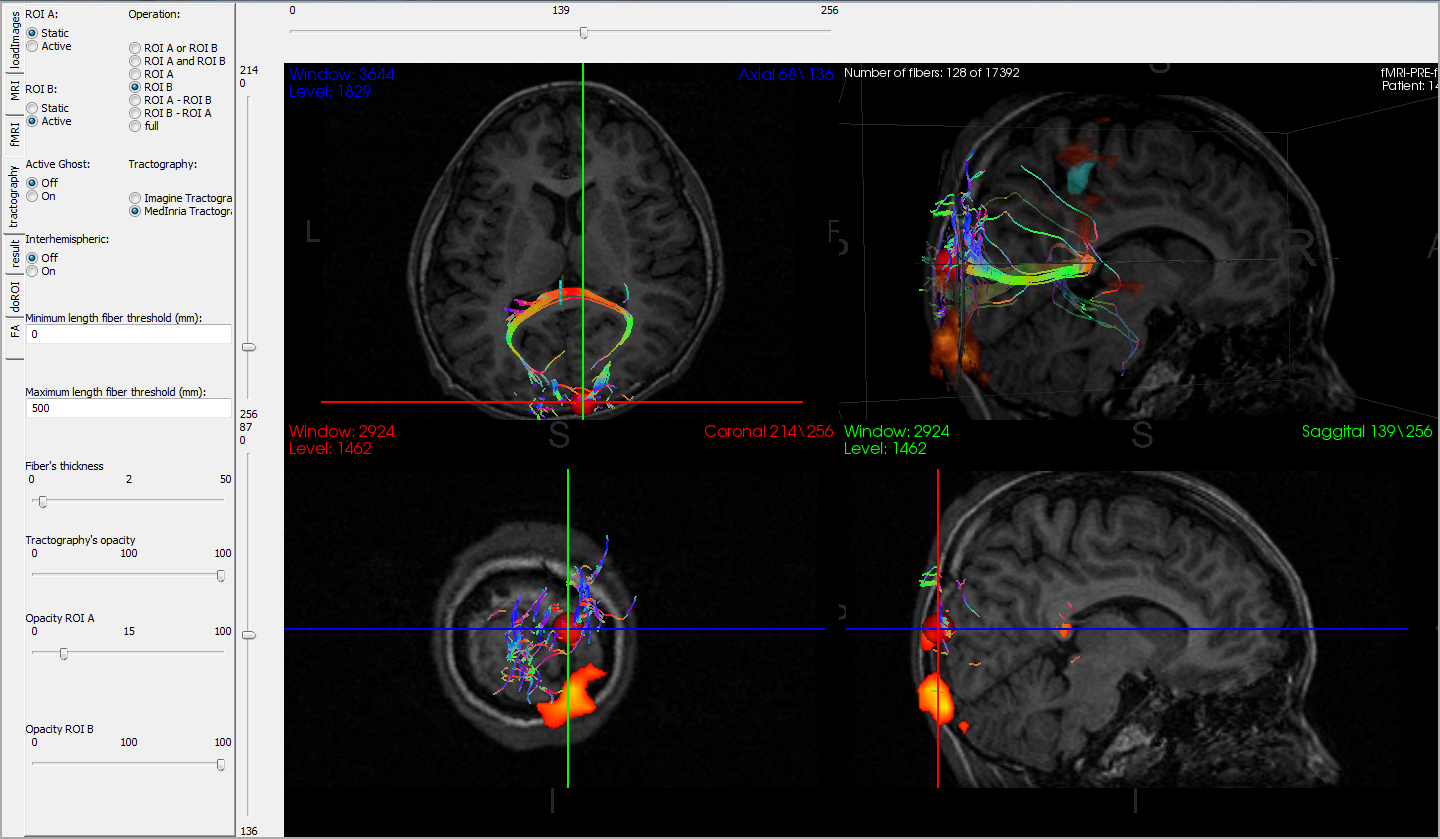
\includegraphics[width=0.9\textwidth]{historic/kab_figura1.png} 
\caption{\label{fig_kab}The main interface of KAB}
\end{figure}

The first prototype built by our group was called KAB \autocite{castro_kab:_2012}. This tool was built to analyze data from the KMC pilot study \autocite{schneider_cerebral_2012}. This software integrated data from Diffusion MRI, Functional MRI and structural MRI. The main interface of the tool is shown in figure \ref{fig_kab}. Data was pre-processed using FSL \autocite{jenkinson_fsl_2012} for skull removal and FMRI modeling, and Medinria \autocite{toussaint_medinria:_2007} for diffusion data. Registration between diffusion and structural spaces was done on-line using the tool itself. The most important features of the software were:

\begin{itemize}
\item Visualizing structural MRI, fMRI and tractography on the same space
\item Selection of bundles in a full tractography
\begin{itemize}
\item Using two spherical regions of interests located manually
\item Using conical regions of interests, representing the spread of TMS magnetic pulses
\item Using areas where fMRI statistics were above a threshold
\item Using hand-drawn regions
\end{itemize}
\item Generating statistics from selected bundles
\item Automatic generation of reports
\end{itemize}

Integrating information from different sources was the major contribution of the tool. Traditionally each type of data was analyzed on its own, using dedicated tools, and integrating information in this way was beyond brain experts. This tool was implemented based on the BBTK framework \autocite{hoyos_creatools:_2012} developed by Creatis. 

Specialists appreciated the ability to integrate several kinds of data and ask questions that involved relationships between them. During the development of the application specialists started asking questions about symmetries in the brain, and therefore the option of reflecting a ROI to the other hemisphere was added. Specialists also expressed the need of linking the coordinate system of the tool to a known atlas.

While this tool made evident the interest in integrated analysis of data, it also had some limitations.
\begin{itemize}
\item It required too much manual work, often repeating tasks
\item It had too many features in a single application, which made it complex
\item Manual registration was very error prone
\item It didn't integrate non-image data.
\end{itemize}
Based on these we proposed a new set of prototypes.

\subsection{First prototypes}

%-- titanic

For the first round of prototypes after KAB, we focused on creating tools with a limited set of features, which could run faster and be easier to learn. We stayed with the BBTK framework as it provided us a fast way to iterate. At this stage our main objectives were solving the technical problems we identified in KAB. Specifically
\begin{itemize}
\item Perform registration automatically
\item Integrate non-image data
\item Increase computational performance
\end{itemize}

\begin{figure}
\centering
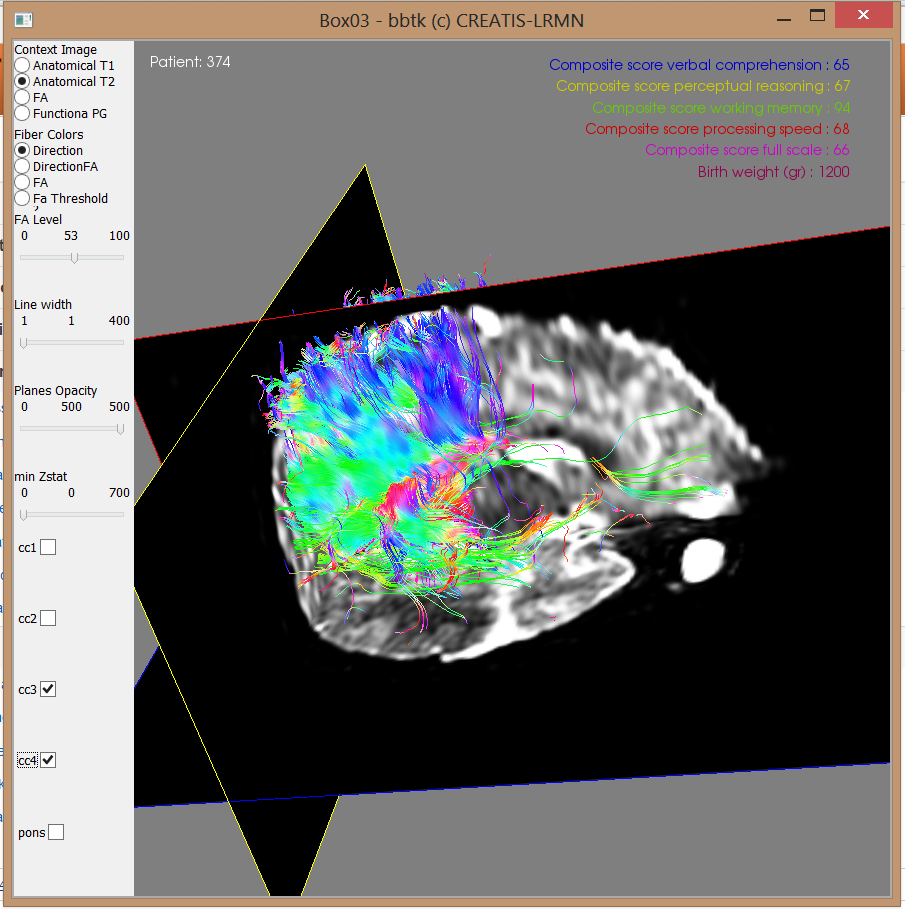
\includegraphics[width=0.9\textwidth]{historic/Titanic_B.png} 
\caption{\label{fig_titanic}Prototype integrating tabular and image data}
\end{figure}

Most of the prototypes created at this stage were only used internally to test different algorithms and techniques. Figure \ref{fig_titanic} shows the final prototype of this series. Its main features are
\begin{itemize}
\item Display values of clinical variables together with the image
\item Explicit identification of the current subject
\item Simple interface
\item Selection of different image modalities
\item Selection of different coloring schemes for bundles
\item Direct selection of the most important fiber groups
\item Control on most important visualization parameters
\end{itemize}

\begin{figure}
\centering
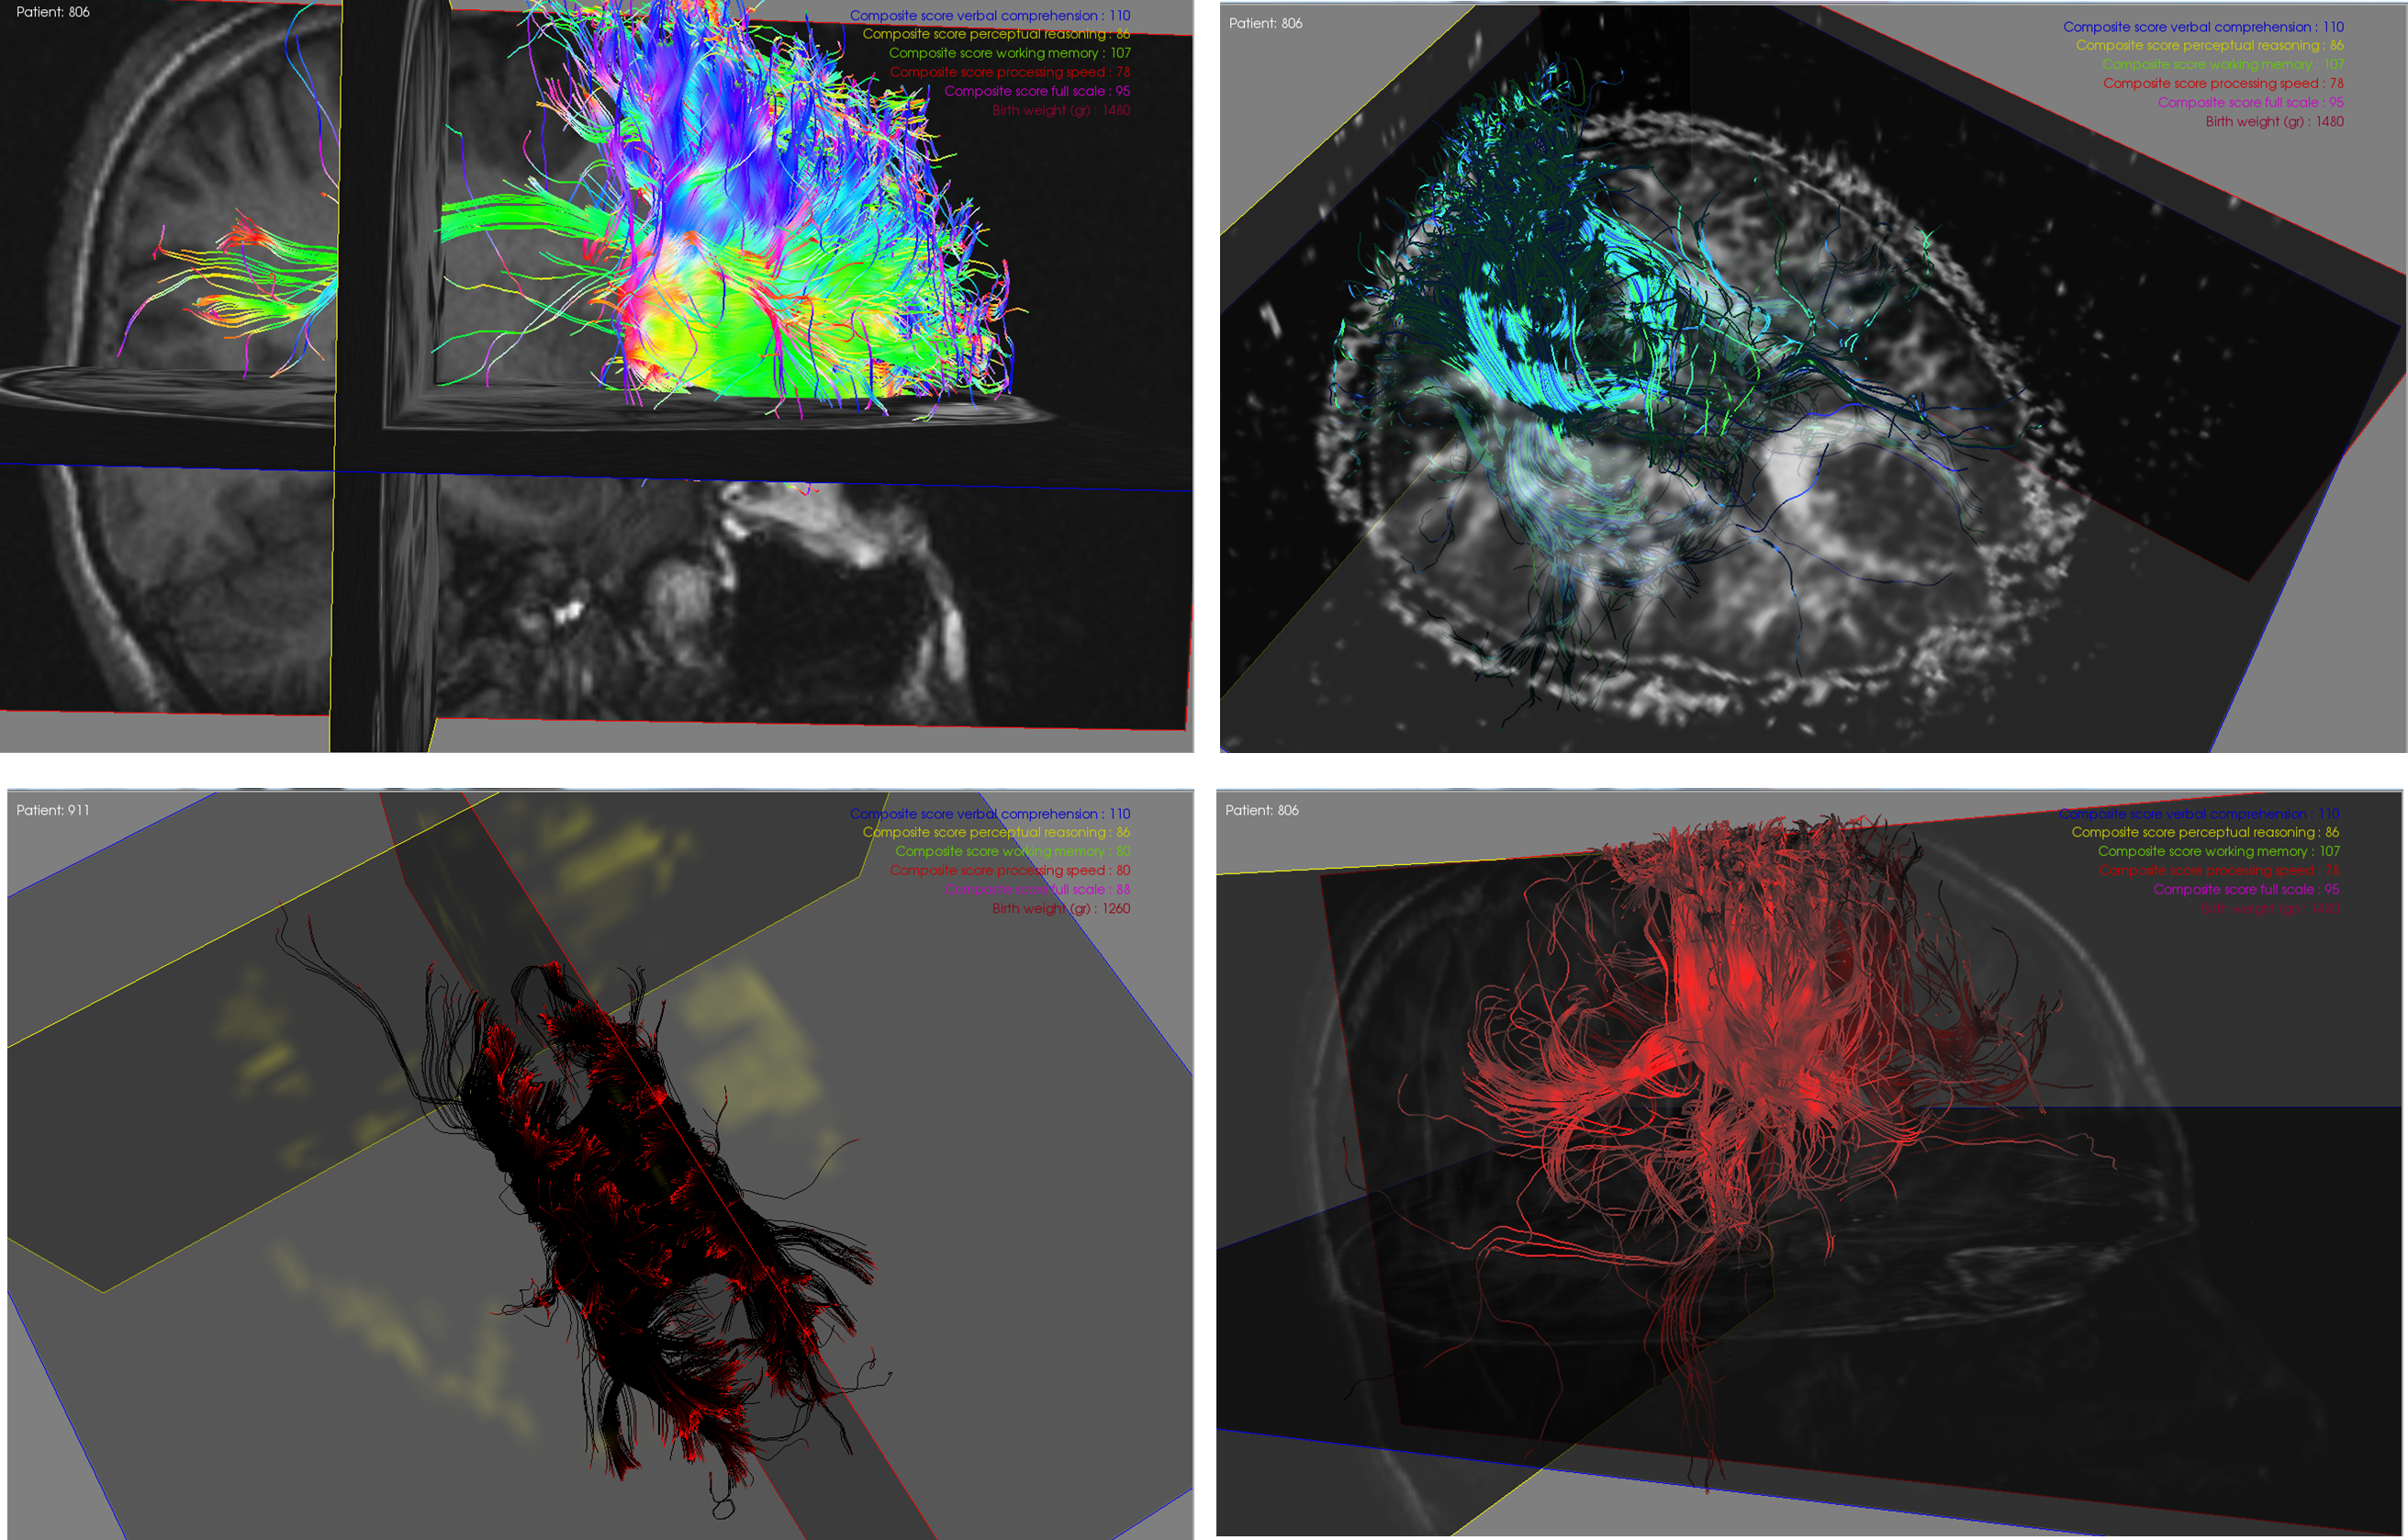
\includegraphics[width=0.9\textwidth]{historic/Titanic.png} 
\caption{\label{fig_titanic_2}The prototype could be configured to show several images and to color fibers in different ways.}
\end{figure}

Figure \ref{fig_titanic_2} shows several of the views that could be accomplished with this tool.
The tool was simple to use as there were few controls and all of them were visible. Notice this application was tailored towards the specific project. At the time the research team was specially interested in corpus callosum and motor fibers. This application allowed researchers to quickly answer specific questions relating fiber bundles to clinical variables. Also now researchers from all specialists could look at tractography and a different MRI images painlessly, where before they had to rely on large, hard to use applications. Data was organized in drive in a well defined structure. When the application launches the user only needed to select the main structural image, and the rest of the necessary files were located trough their relative paths. There was no need for end user to even know about the existence of transformation matrices or other files. This simplified a lot the process of simply looking at spatial data in context, and allowed experts to do this in a convenient way. Having a more direct access to spatial data allowed experts from different specialties to look at them on their own time, and therefore come up with new ideas for analyzes. They were also using the tool to communicate ideas to other brain experts and also to us. We now had a better way of communicating with experts, and therefore we could get a better understanding of their needs. This tool showed us the potential of integrating spatial data with clinical data, but some limitations were made evident in our work with experts
\begin{itemize}
\item It was not possible to change subject during an analysis
\item It was not easy to select different variables
\item It was not possible to use different sets of tracks
\item It is cumbersome to compare different subjects
\end{itemize}

Analyzing groups of subjects and comparing subjects became the priority for the next round.

\subsection{Braviz, First Version}

%- Braviz/tk
%-- sample applications

For the next cycle we dropped the BBTK platform as we found out it was limiting too much our design space. The platform enforced an execution model that kept everything updated. This was great for small applications, that were meant to run for just a couple of minutes. However for large applications that could run for hours we required more control of when the different modules would execute. BBTK relied on VTK for all visualization tasks, and therefor we decided to start developing directly on VTK. However it was still very important to us to have quick development cycles, and we were willing to sacrifice some performance to get it, therefore we switched our main developing language to python. In the following we will describe some of the applications developed at this stage. 

We were exploring how to bring into the applications of more sophisticated processing tools. FreeSurfer specially grabbed our attention as it provided information from an ATLAS, and provided a way to identify the different regions of the brain using common names. This was very important to experts as it allowed them to compare their finding to those of other groups, and those in the literature. Figure \ref{fig_surf_1} shows one of the prototypes which allowed experts to visualize FreeSurfer surface parcellations. This application has a 3D viewer on the right side and a control panel on the left side. The bottom part of this panel lets the user select the different FreeSurfer surfaces and scalars, while the top of the panel lets him show a subject. Notice that it is now possible to change the subject in the middle of a session, and by doing so, it is also easier to compare the same view for multiple subjects. This was one of the main goals at this stage. 

\begin{figure}
\centering
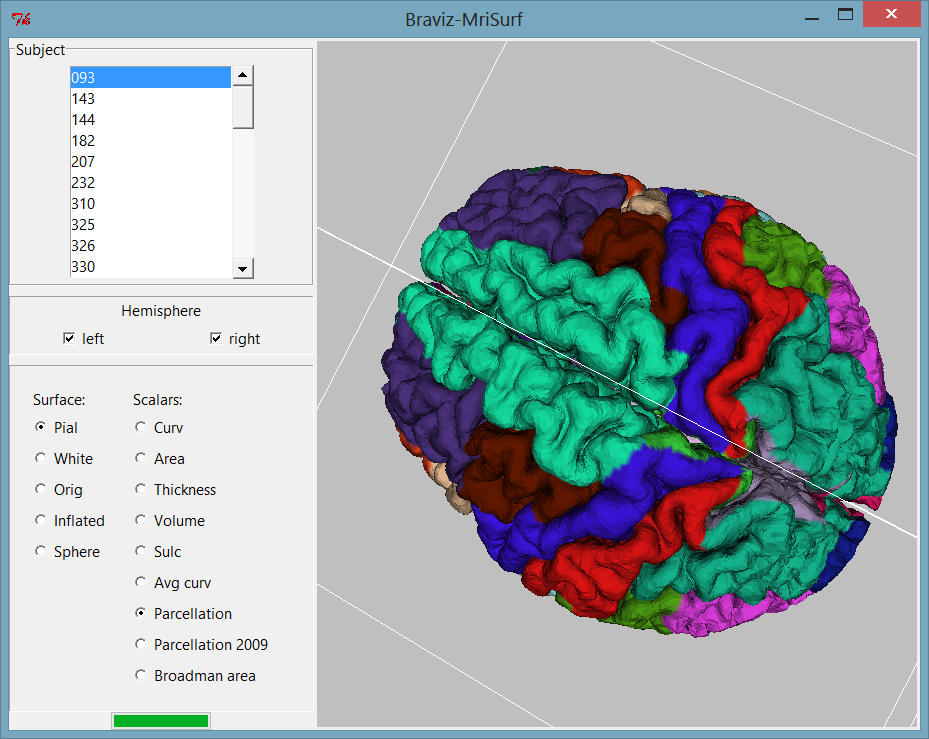
\includegraphics[width=0.9\textwidth]{historic/surf1.png} 
\caption{\label{fig_surf_1}A freesurfer surface inside Braviz}
\end{figure}

The FreeSurfer segmentations also provided us a repeatable way of selecting fibers across all subjects. Figure \ref{fig_cc_ctx_1} shows an application designed for this task. In the control panel we now have a list of structures where the user can select one or several. In the middle of the panel is a combo-box which provides the options "\emph{or}" or "\emph{and}". This selection will change the way in which multiple selections are interpreted, in the case of \emph{or}, fibers that go trough any of the structures will be selected, while in the case of \emph{and} only fibers that go trough all of them will be selected. Notice there is another combo-box labeled "\emph{coordinates}", this box provides the options "\emph{world}", "\emph{talairach}" and "\emph{dartel}". In "\emph{world}" objects on the 3D view are represented based on the coordinates of the anatomical image, in "\emph{talairach}" mode the coordinates change to the standard Talairach space and, in "\emph{dartel}" mode, objects are registered to sample template using a non-linear registration. By moving to a standard space comparing two different subjects is easier, as some of the differences will be absorbed by the transformation. This will enhance some types of differences but will hide some others; the most appropriate coordinate system will depend on what types of differences are currently of interest for the end user. In this application several other FreeSurfer structures could be added to the scene in order to provide context. Figure \ref{fig_fibers_ctx} shows another view of this application. By hovering the cursor on top of a bundle the user could get some information about them. It was also possible to measure distances in the 3D space in order to make numeric comparisons across subjects.

\begin{figure}
\centering
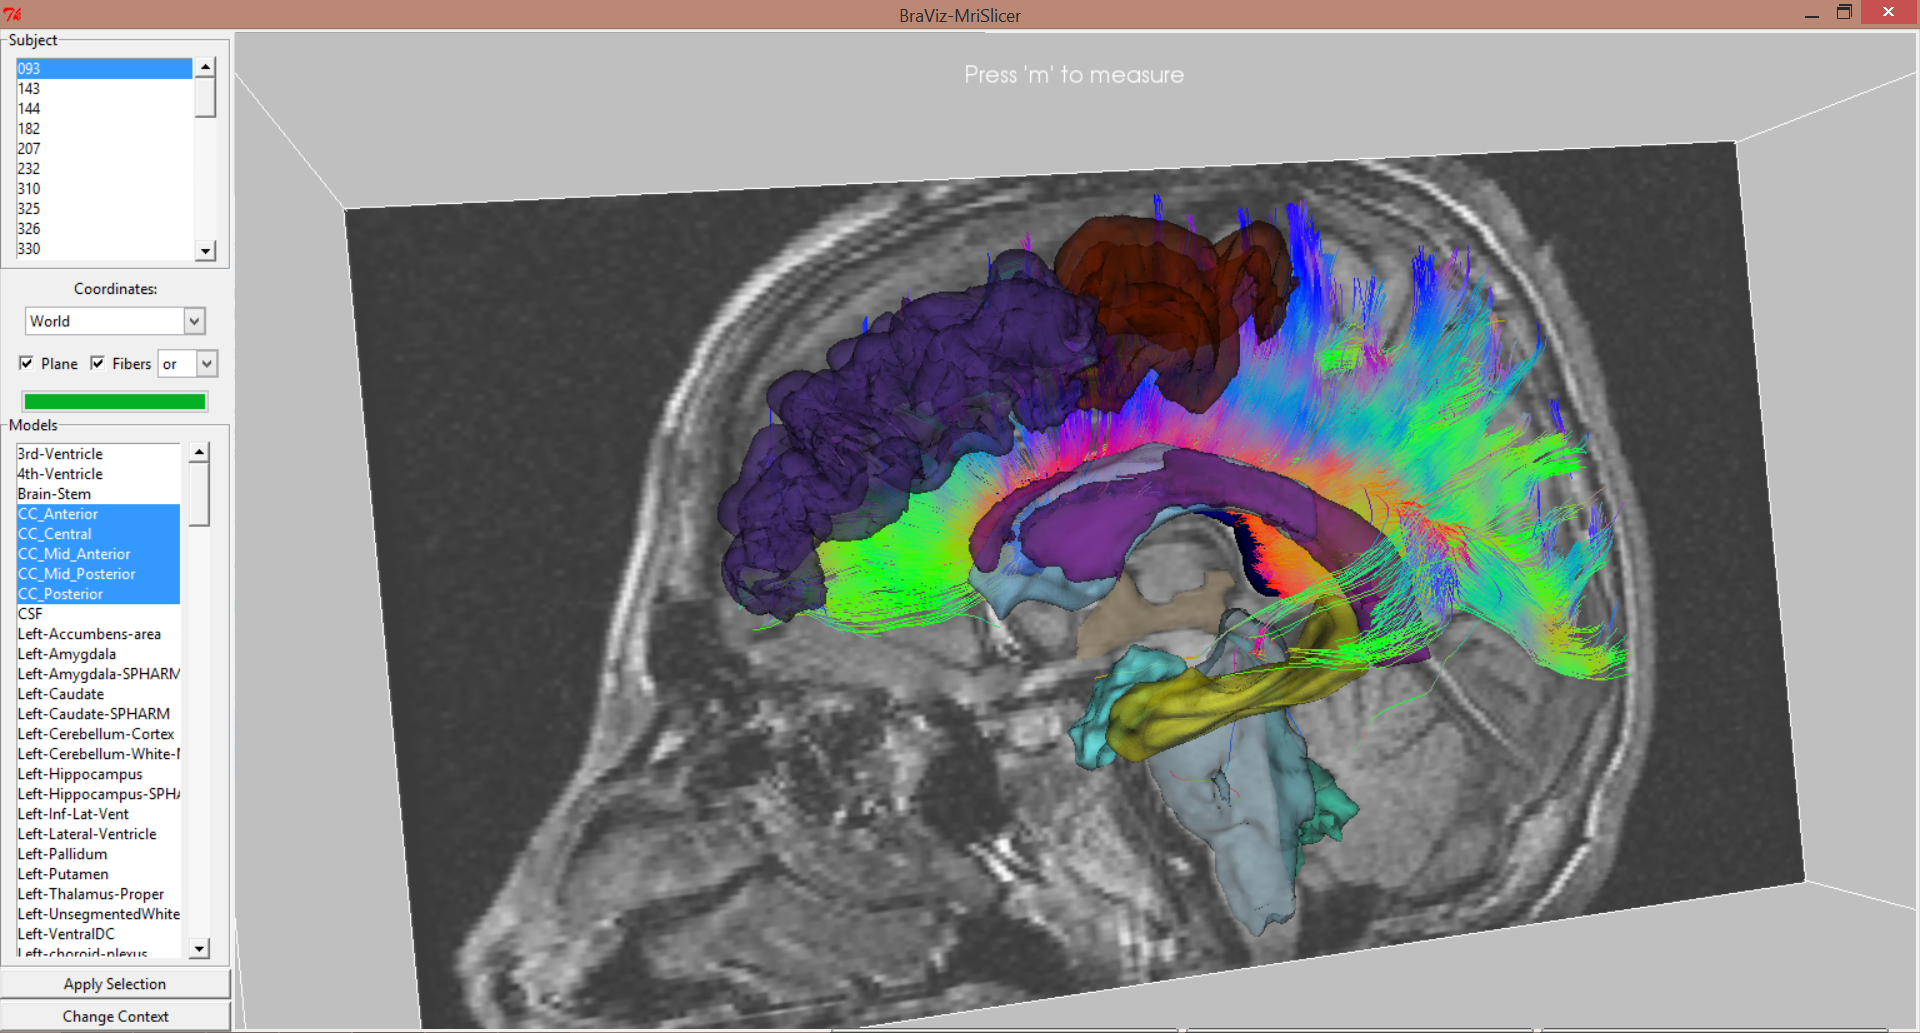
\includegraphics[width=0.9\textwidth]{historic/cc_in_context.png} 
\caption{\label{fig_cc_ctx_1}Fibers of the corpus callosum with segmentation and anatomical image as context}
\end{figure}

\begin{figure}
\centering
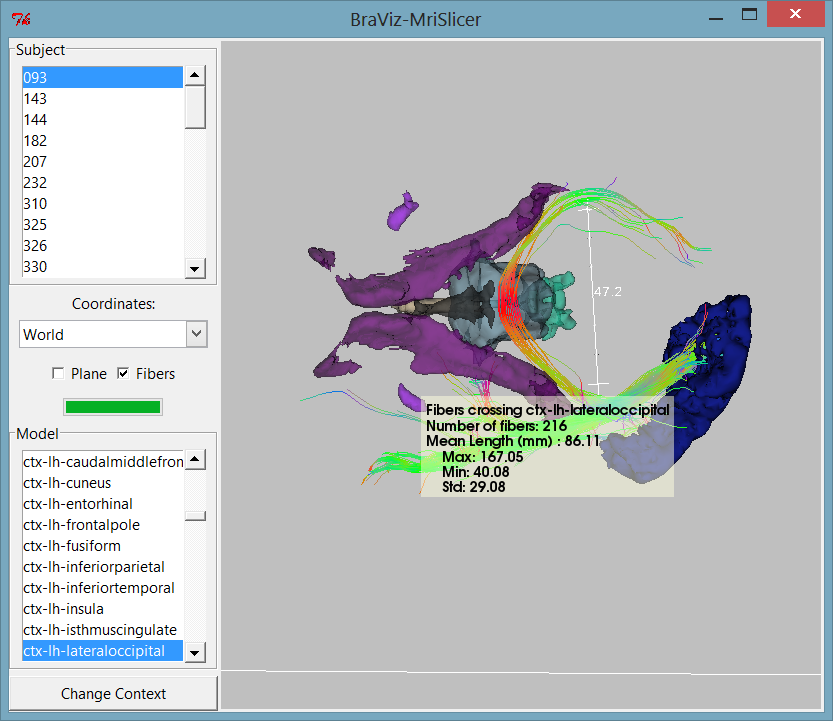
\includegraphics[width=0.9\textwidth]{historic/fibers_in_context.png} 
\caption{\label{fig_fibers_ctx}Fibers could be selected using freesurfer segmentation. Vtk widgets could be used to make measurements.
Additionally statistics of each bundle were also available.}
\end{figure}

An application for viewing two subjects at the same time and comparing them was also created. Its interface can be seen on figure \ref{fig_compare_1}. In this application it was possible to show the same selection of images, fibers and structures for two different subjects. The screen could be split vertically, horizontally or both subjects could be shown on the same space but using different colors and possibly adding a small offset. In the case of split screen the camera in both views was coordinated, and there was the possibility to add a plane that would be replicated in both views to use as context.

\begin{figure}
\centering
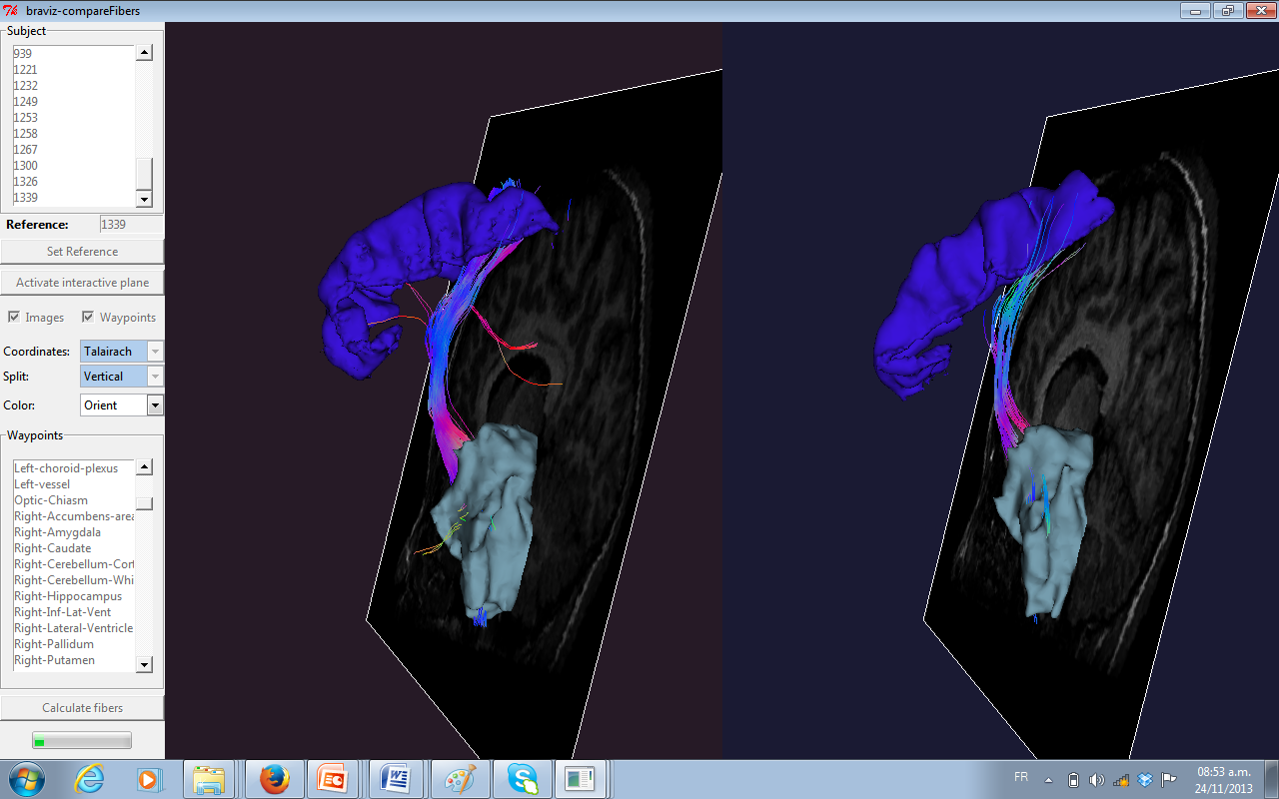
\includegraphics[width=0.9\textwidth]{historic/compare.png} 
\caption{\label{fig_compare_1}Comparing the motor tract of two subjects}
\end{figure}

At this point the interest in fMRI was increasing, but some of the researchers who were not expert on this technique were having problems interpreting this data correctly. Figure \ref{fig_fmri_1} shows an application created to make the nature of fMRI explicit. The application shows the T-score image in the 3D view, but also shows the corresponding time signal at each voxel, together with the experiment design. In this way users could better understand that a higher score meant a larger relationship between the BOLD signal an the paradigm. 

\begin{figure}
\centering
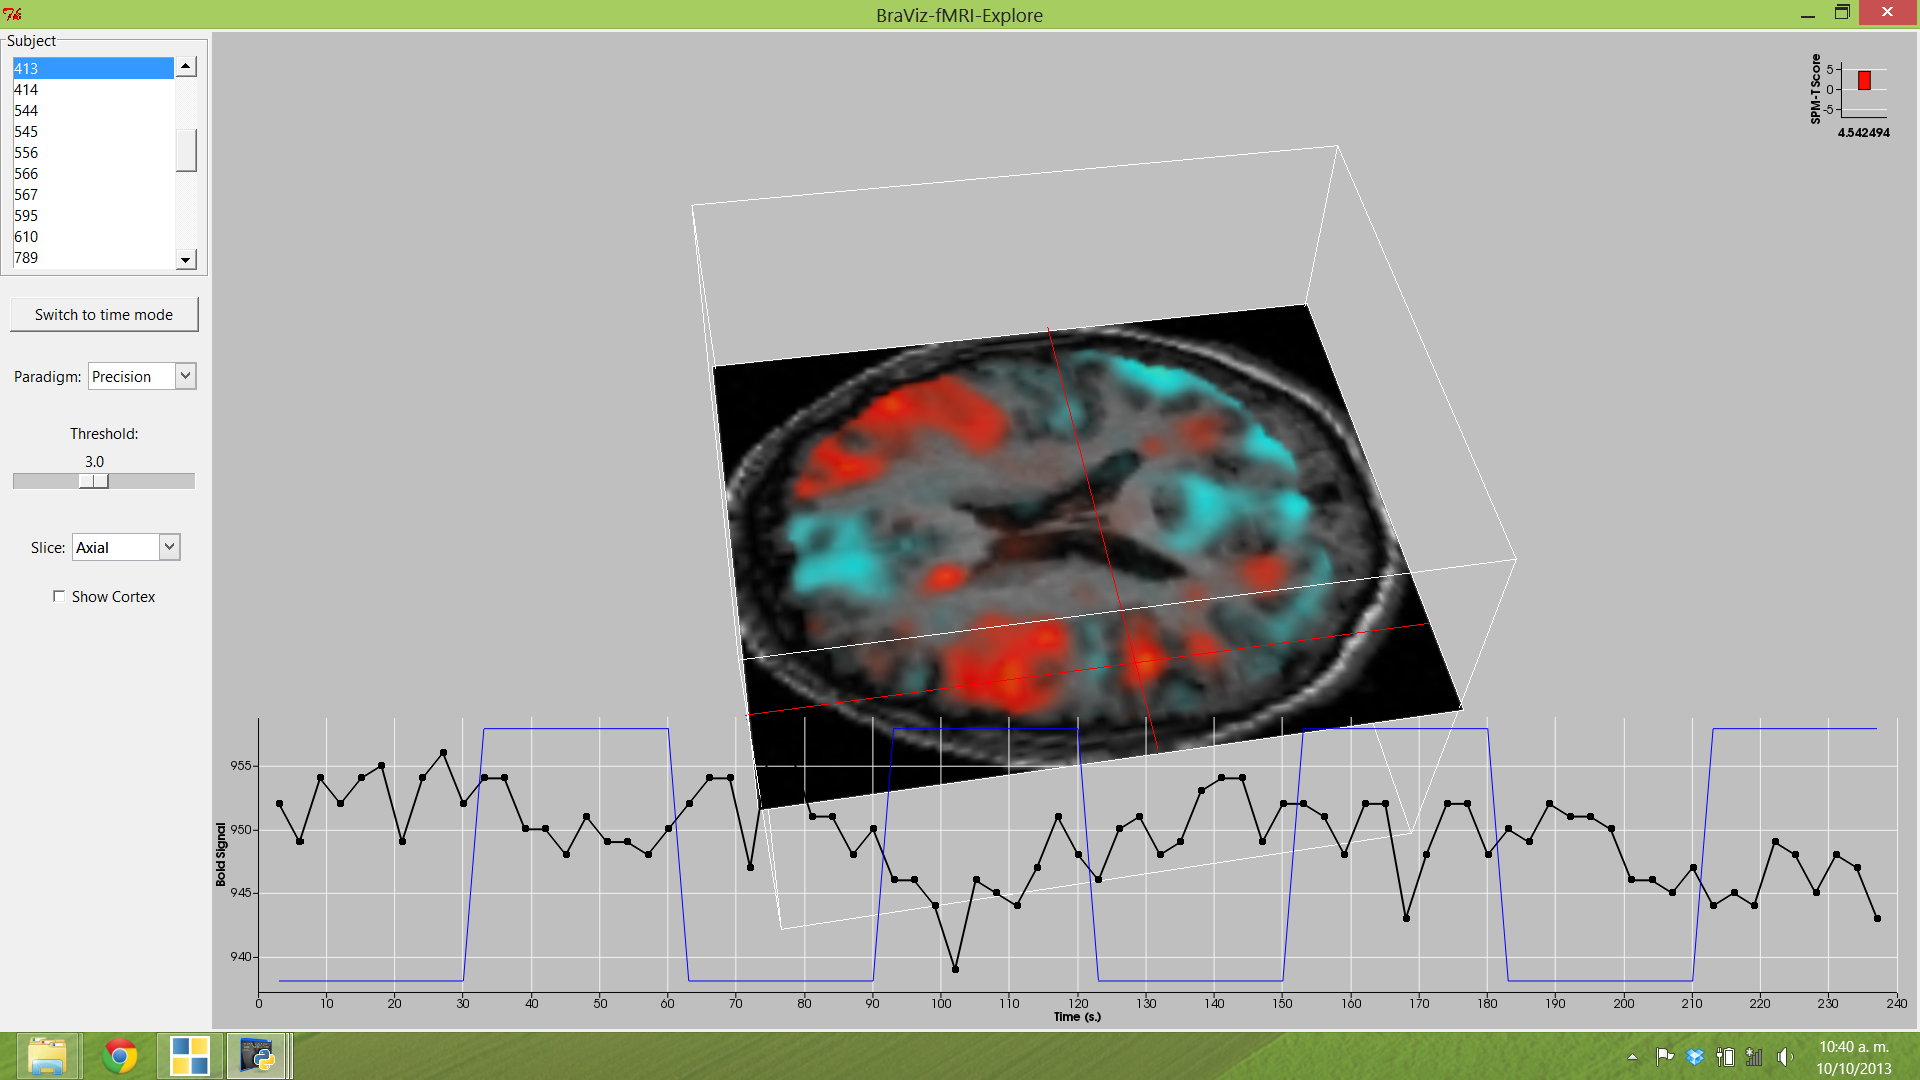
\includegraphics[width=0.9\textwidth]{historic/rejean2.png} 
\caption{\label{fig_fmri_1}This prototypes make the time dimension of fMRI explicit, therefore helping non-experts understand its meaning and make better interpretations}
\end{figure}

We wanted to let researchers search for patterns between clinical variables and structures. One proposal in this direction can be seen in figure \ref{fig_grid}, this application shows the corpus callosums of all subjects in the study organized in a grid. From left to right the structures are organized according to a clinical variable, while the color of the structures reflect the value of another clinical variable. The variables used for these purposes could be selected from the panel on the left. At the bottom right of the viewer was a small scatter plot showing the relationships between the two variables. This plot was linked to the grid view, so selecting a point in the plot would highlight the corresponding structure and vice versa. Another important feature was that an individual structure could be rotated in 3d space, and the rotations would be propagate to all the structures on the grid.

\begin{figure}
\centering
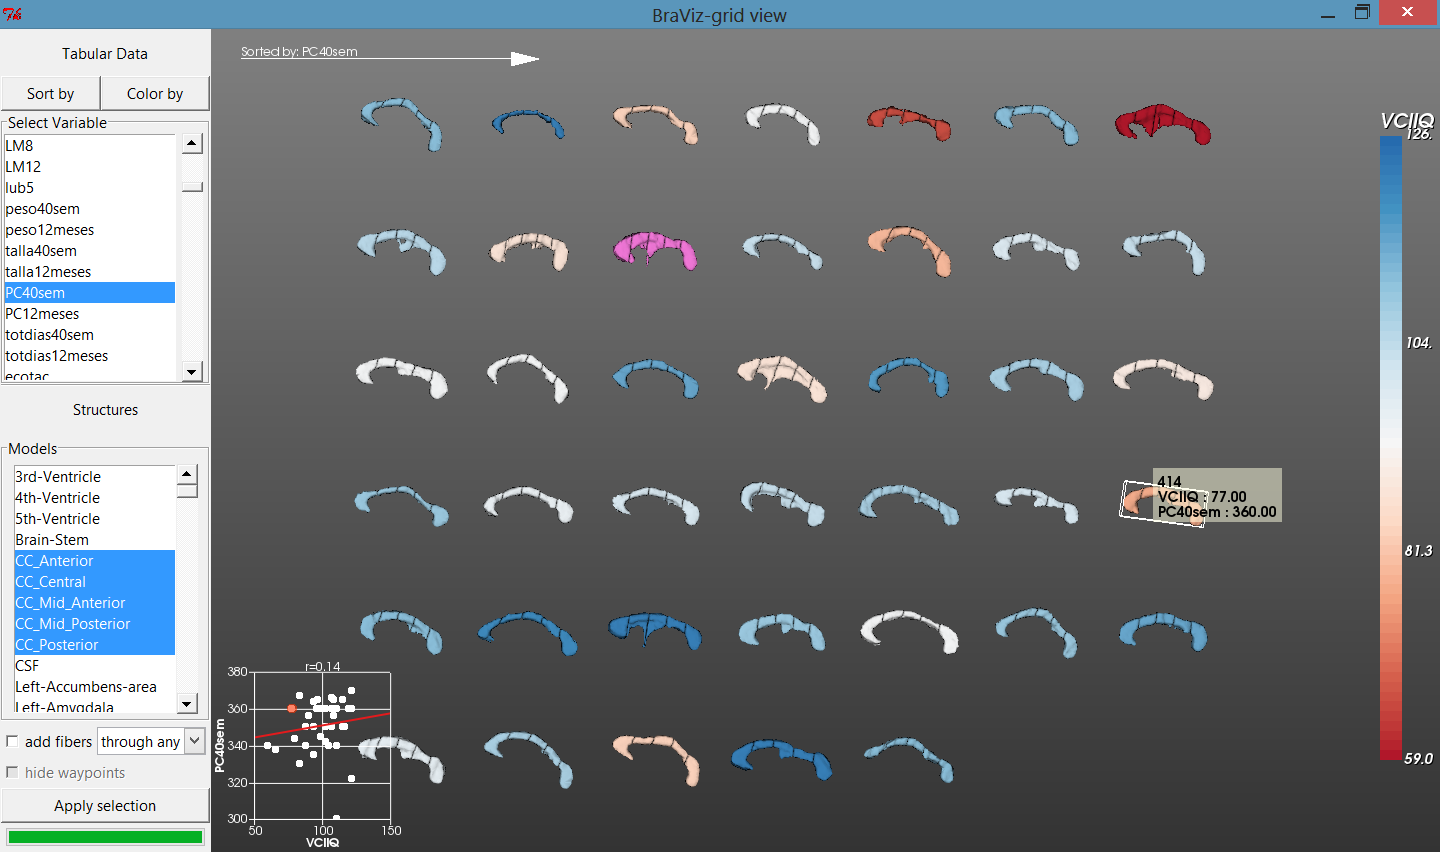
\includegraphics[width=0.9\textwidth]{historic/grid_and_scatter.png} 
\caption{\label{fig_grid}Corpus Callosums of several subjects organized on a grid and colored with respect to clinical variables.
A scatter plot of these variables is shown at the bottom left}
\end{figure}

Another proposal for showing relationships between structures and clinical variables is shown in figure \ref{fig_star_1}. In this case structures and data are separated in three groups. This grouping is done by the main categorical variable in the study (see chapter \ref{chap_kmc}). Clinical data is shown using a spider plot, where each subject is represented as a polygon and each variable is an axis. Structures are shown on the same space using alpha-blending. By mixing all the structures in this way the average shape for the group appears. Also notice variables are organized in a tree like structure on the top left, and the description of each variable appears when the user hovers on its name. This tree also showed FreeSurfer structures and allowed the user to add the volumes and areas of such structures to the star plot. As in the previous case there was an integration between the numerical variables and the structure, and clicking on one would highlight the corresponding subject on both views.

\begin{figure}
\centering
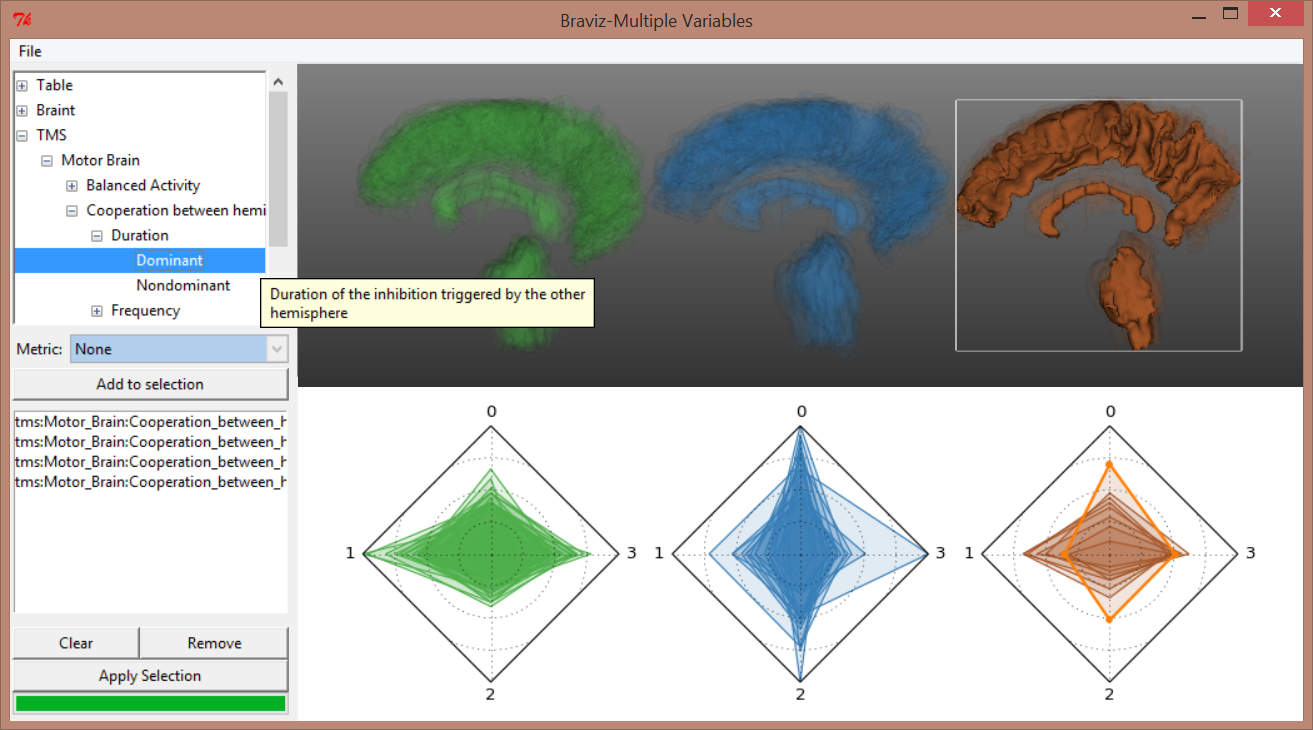
\includegraphics[width=0.9\textwidth]{historic/mini_star.png} 
\caption{\label{fig_star_1}This application allowed comparing several structures and variables between groups of subjects.}
\end{figure}

The application shown in figure \ref{fig_tms_1} was developed for a very specific task: analyzing the relationship between TMS metrics with fibers. The application shows at the left a list of tms variables organized in a tree, a selection between dominant and non-dominant hemisphere, and the option to add males or females to the sample. In this case the application would know if a given subject is right handed or left handed, and display the values for the dominant or non-dominant hemisphere. At the bottom of the screen the values for the whole sample would be shown with the current subject on the right. The picture at the top of the screen would display the motor fibers where the current metric only involved one hemisphere, and the corpus callosum (see figure \ref{fig_tms_2}) where the current metric involved both hemispheres. The user could click on a bar on the bottom display and select that subject.
It was also possible to show aggregated measures for the three groups on the bottom display as seen in figure  \ref{fig_tms_2}. By doing this the expert could quickly evaluate the relationship between the visual appearance of tractography and values of tms metrics. 

\begin{figure}
\centering
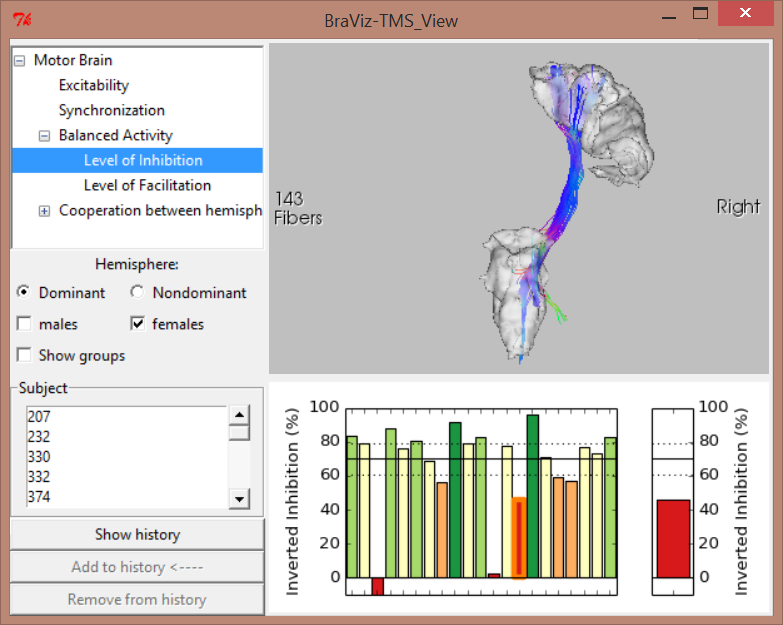
\includegraphics[width=0.9\textwidth]{historic/mini_tms.png} 
\caption{\label{fig_tms_1}An application tailored at analyzing TMS variables relationship with tractography}
\end{figure}

\begin{figure}
\centering
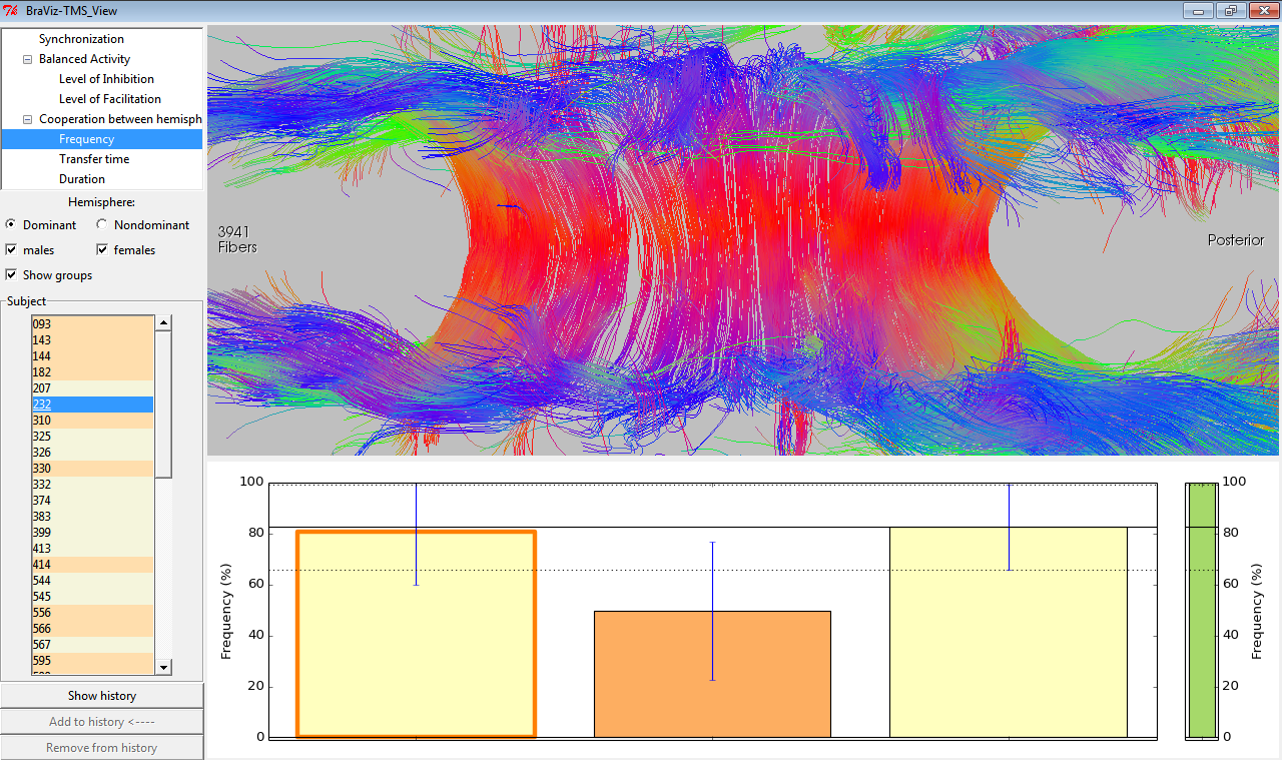
\includegraphics[width=0.9\textwidth]{historic/tms_2.png} 
\caption{\label{fig_tms_2}Another view of the TMS applications, this time showing the fibers of the corpus callosum.}
\end{figure}

Finally, we created a menu in order to group all applications and provide users with a direct access point to all of them. Before this, we had a collection of icons in a folder, but users found it complex. Trough the menu they can see a picture of each application, and therefore find the one they need without even reading.

\begin{figure}
\centering
\includegraphics[width=0.9\textwidth]{historic/braviz_menu.png} 
\caption{\label{fig_menu_1}A menu was provided to give an overview of the available applications and provide simple access.}
\end{figure}

By this iteration we had more confidence in the underlying data analysis steps, and therefore were able to propose a wide array of solutions. We got closer to our goal of analyzing groups of subjects and integrating clinical variables with structural data. The features users liked the most were

\begin{itemize}
\item Seeing the same display for different subjects
\item Associating locations in the image to areas in an Atlas
\item Relating Volumes, Areas and Lengths of fibers to clinical variables
\item Quickly seeing relationships between clinical variables
\end{itemize}

As it can be seen the interest in the analysis of clinical values was increasing. In fact the favorite feature from the grid viewer in figure \ref{fig_grid} was the scatter plot at the corner. We were somehow disappointed for the lack of interest in the 3D graphs, but those were the opinions of the users. In fact they mentioned that hardly anything could be seen in the alpha blended images from figure \ref{fig_star_1}. In other views they were happy to be able to see the data, but they demanded even more for numerical measures where statistics could be applied. Therefore the main goal for the next iteration was improving the support for clinical data.

%Feedback

\subsection{Braviz, Second Version}

%- Braviz Qt
%-- sample applications

The first version of Braviz provided a robust infrastructure for displaying spatial data on multiple coordinate systems, however its ability to handle clinical variable was still limited. From the last iteration we realized that in order to efficiently use the data we needed some analytics on the variables. We also required a better infrastructure to store and manipulate this variables. Another limitation of the previous prototype was that work could not be saved or restored. Measurements derived from segmented structures or fibers were separated from clinical variables. Finally, all of the applications operated independently without any connection. This version of Braviz addresses those limitations. 

In order to store and manage clinical variables and those derived from spatial data a database was integrated in the system. This database is also used to let user store and retrieve data. Details of the database will be given on section \ref{sec_tech}. Applications were coordinated by sharing the same database, and by passing messages between them. The model described in chapter \ref{chap_model} was mature by this moment, and was the basis for this implementation. Section \ref{sec_arch} will provide a closer look at how the model is realized into this platform, but first we will take a look at some of the features of this version.

\begin{itemize}
	\item Centralized storage of variables and user data
	\item Importing and Exporting variables to/from spreadsheets
	\item Coordinated applications, can focus on the same subject on all applications
	\item New QT based user interface
	\item Create new variables based on spatial data and add them to the database
	\item Statistical processing based on R
	\item Create, use and share custom sub-samples
	\item Save and restore the state of applications
\end{itemize}

We took all of the different data viewers of the previous iteration and combined them into a single viewer, called \emph{subject overview}. This viewer can be used to show all the different kinds of data that are available on the same space. Several of the possibilities are shown on figure \ref{fig_subj_viewer_mosaic}. The main interface of this application is shown in figure \ref{fig_subj_overview_2}. Notice that below the main view now we can find the values of several values for the current subject. Another feature is that the viewer lets the user calculate scalar metrics based on the objects in the scene, and add this values to the database as a new variable.

\begin{figure}
\centering
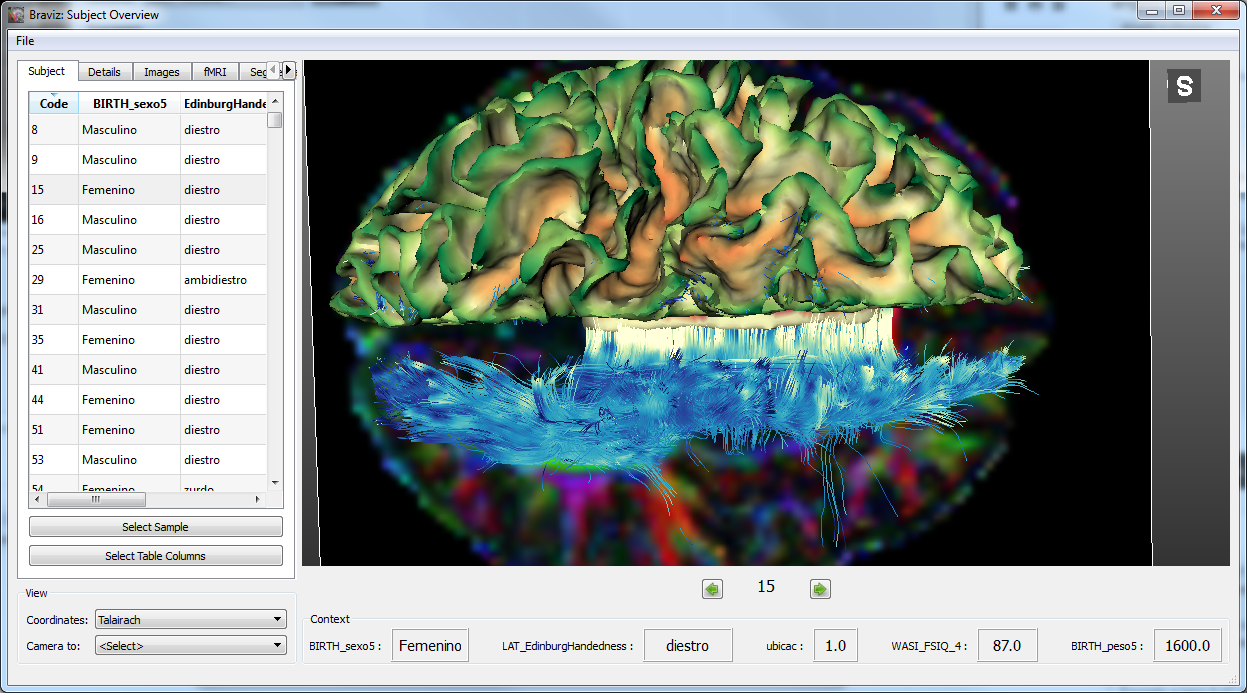
\includegraphics[width=0.9\textwidth]{braviz_qt/subj_overview_full.png} 
\caption{\label{fig_subj_overview_2}The new subject viewer integrates all of the data-types from previous version on the same application, therefore allowing all types of combinations.}
\end{figure}

\begin{figure}
\centering
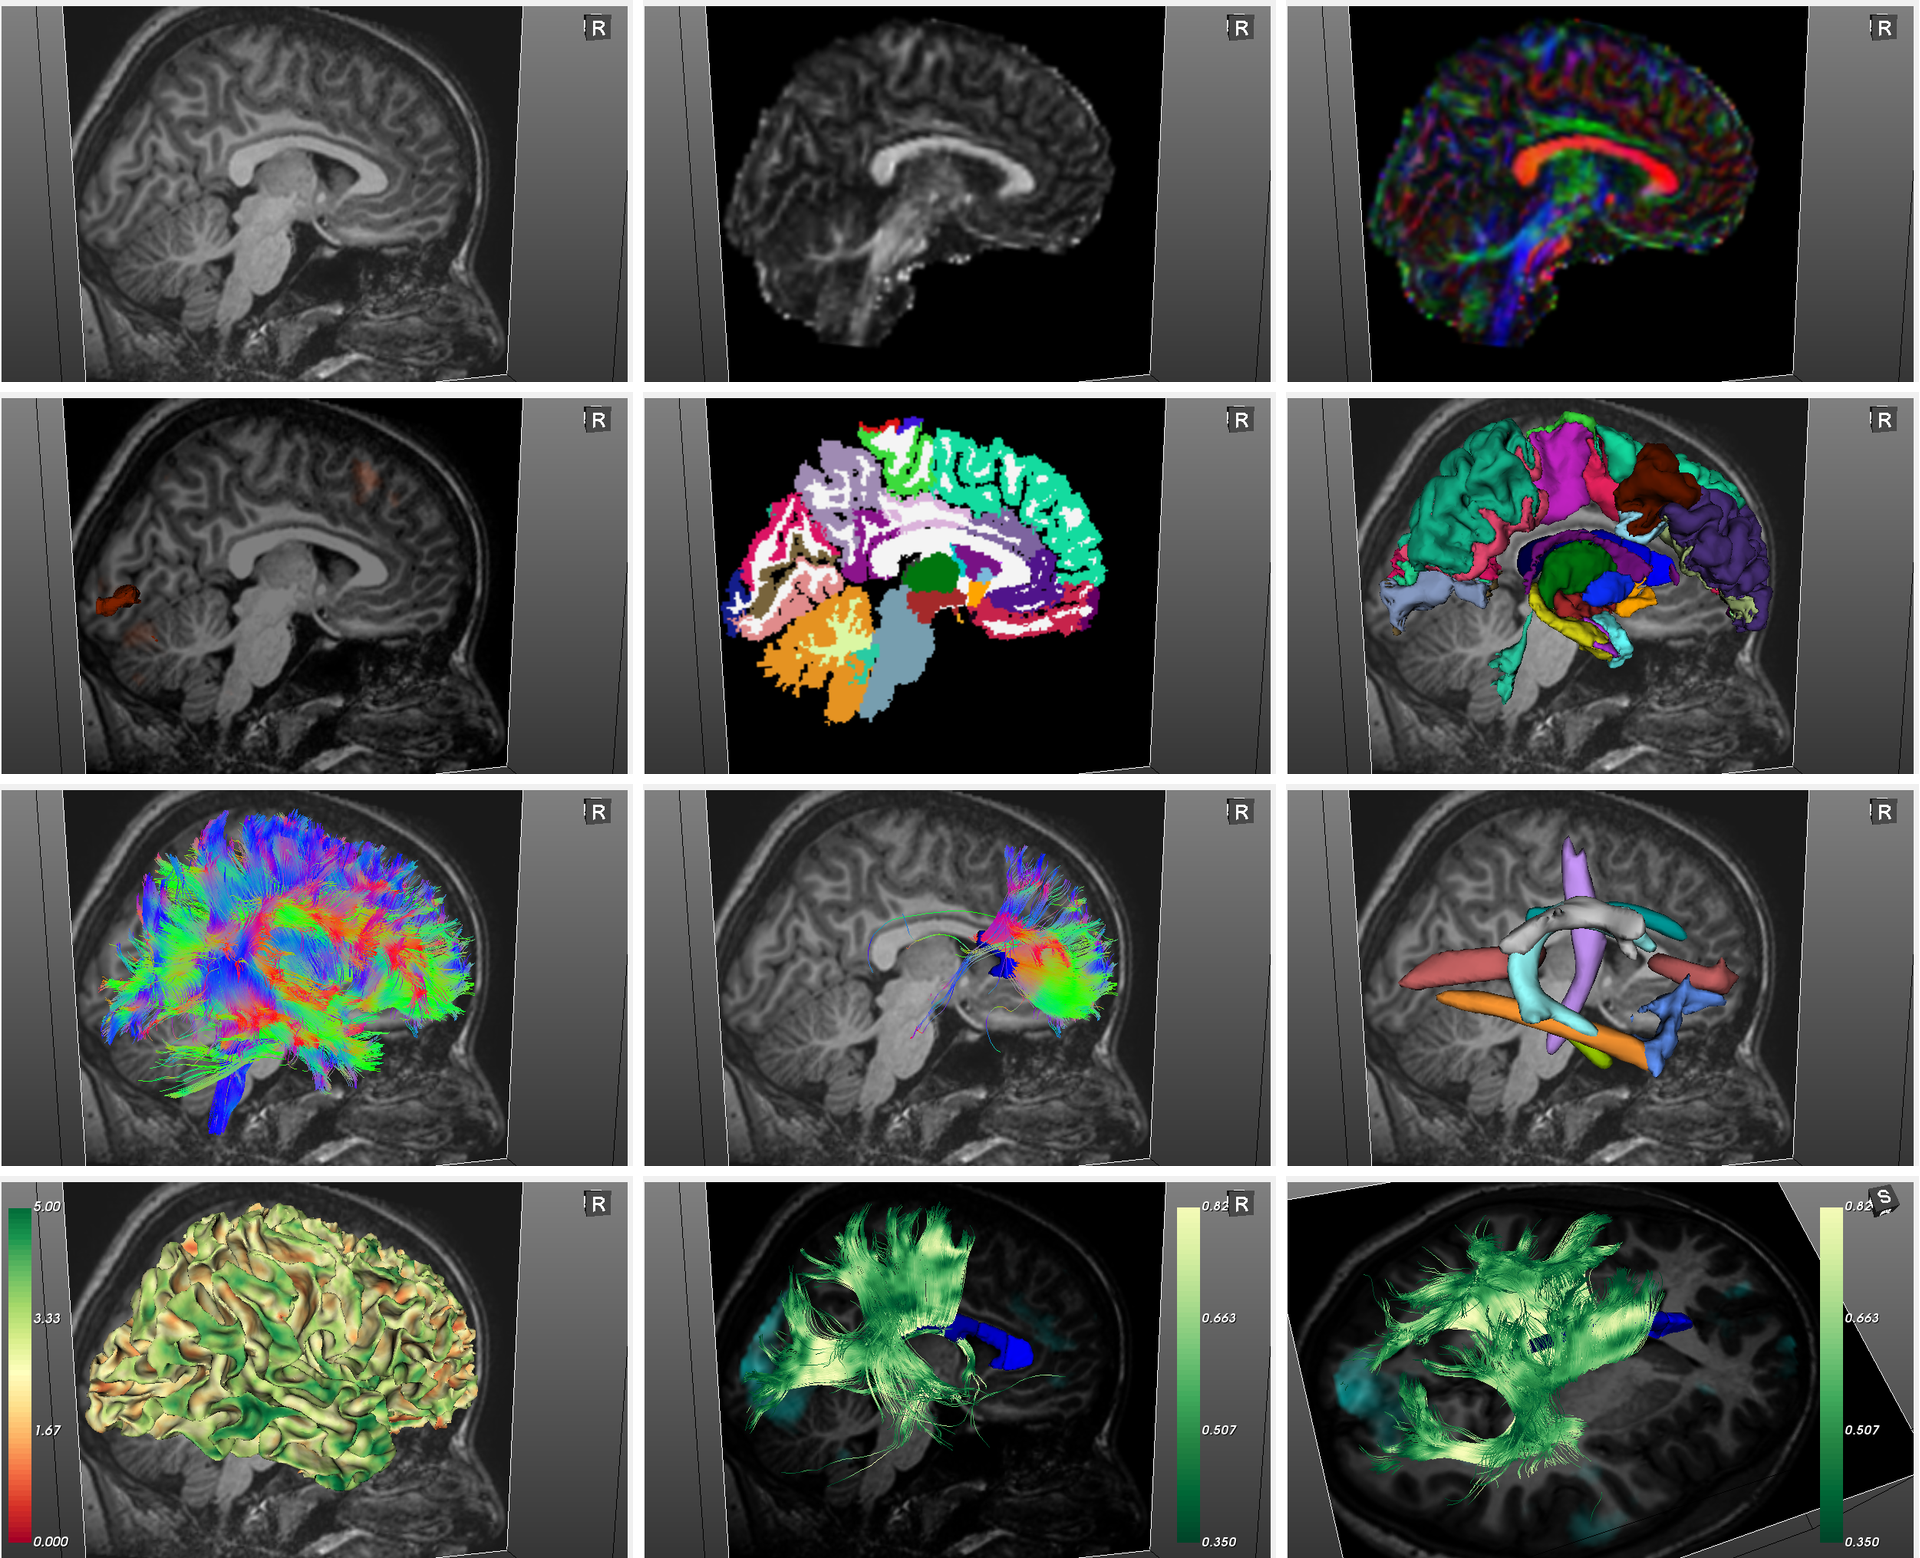
\includegraphics[width=0.9\textwidth]{braviz_qt/subj_viewer_mosaic.png} 
\caption{\label{fig_subj_viewer_mosaic}Examples of visualizations that can be achieved with the new subject viewer.}
\end{figure}

The application shown in figure \ref{fig_sample_overview_2}, called \emph{sample overview}, lets the expert look at several subjects at the same time. Subjects are arranged in rows based on a nominal variable and from left to right based on a numerical value. The values of this variables are also shown on the bar plots at the right. Each bar is linked to one 3d viewer, and by selecting a subject on one of the view it will be highlighted on the other one. As before it is possible to manipulate the camera on one viewer and copy it to the rest. Notice that we abandoned the idea of alpha blending in favor of multiple views that we expect will be easier to interpret. If more details from a single subject are required, the user can right click on the small picture, and from the context menu select \emph{show in other viewers} or \emph{show in new viewer}. The first option will highlight the subject on all opened viewers, while the second one will launch a new subject overview subject configured in the same way as the small viewer.

\begin{figure}
\centering
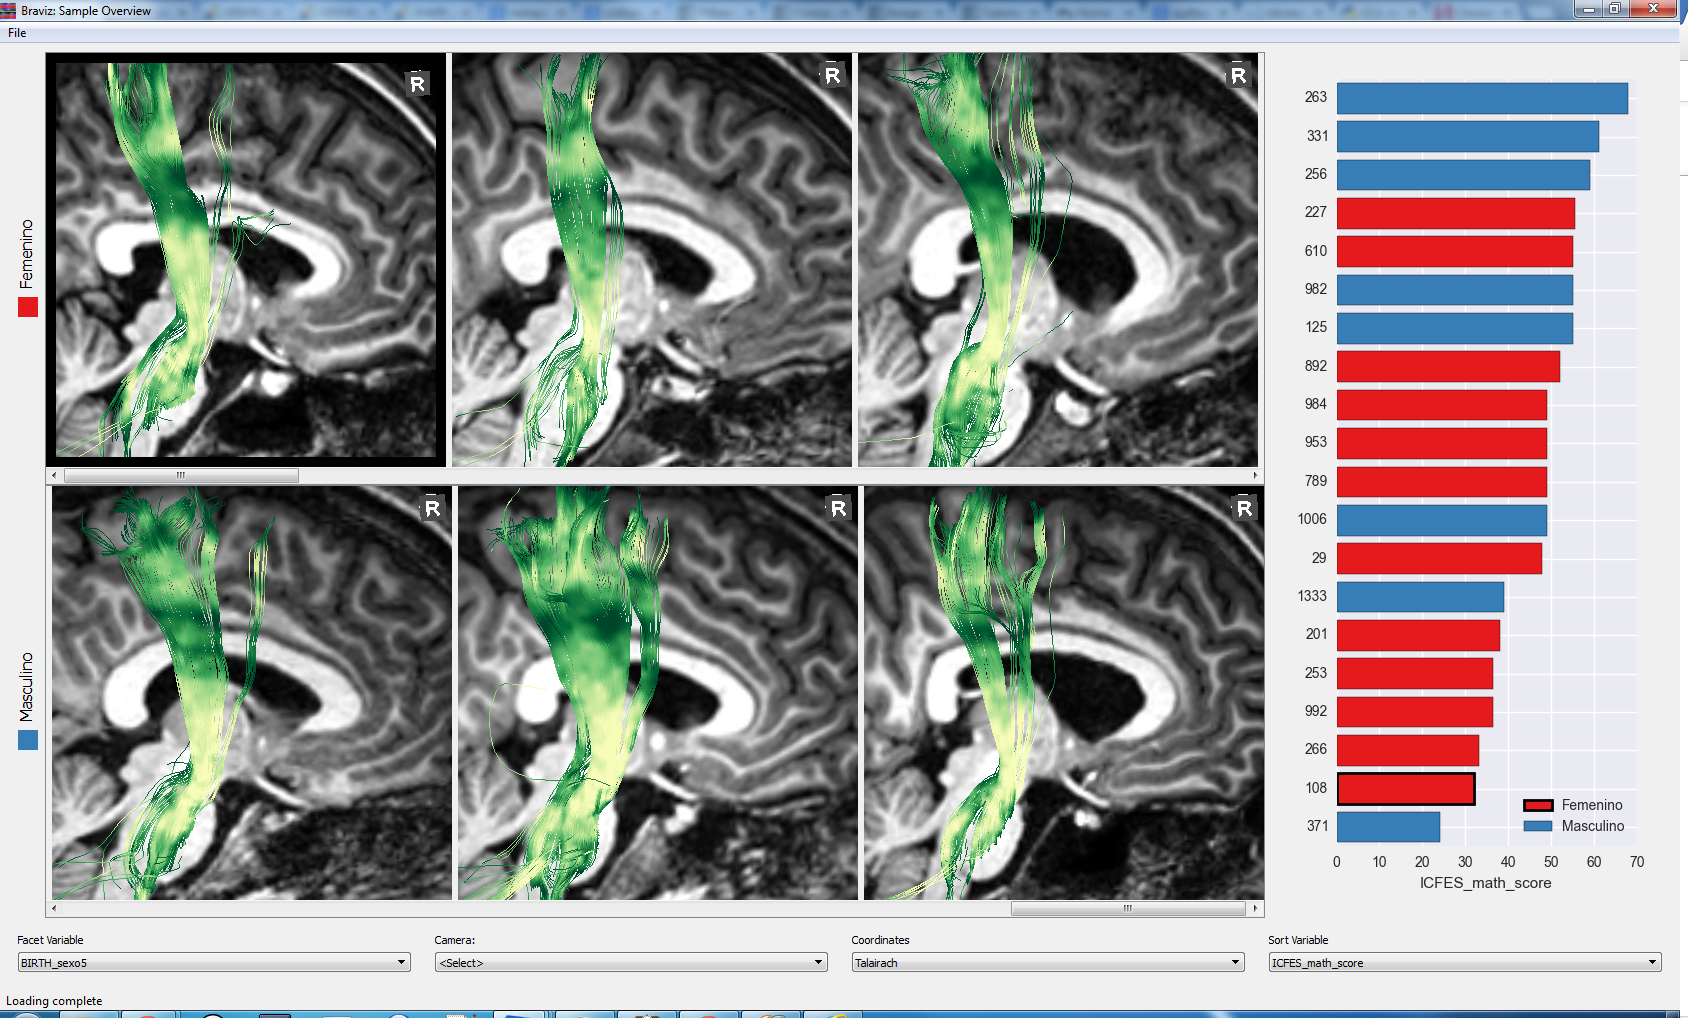
\includegraphics[width=0.9\textwidth]{braviz_qt/sample_overview.png} 
\caption{\label{fig_sample_overview_2}Multiple subjects can be visualized at the same time in small multiples, a nominal variables is used for rows and a numerical value for left to right order.}
\end{figure}

In order to select variables in all of the applications, dialogs similar to the one shown on figure \ref{fig_var_select}. This dialog shows a list of variables that can be filtered, and for each variable provides a description, a type and a plot. In the case of nominal variables the labels for each level are also shown, while on numerical value the expected range of the variable and the optimal value is shown. Notice that this information can be modified by the user. 

\begin{figure}
\centering
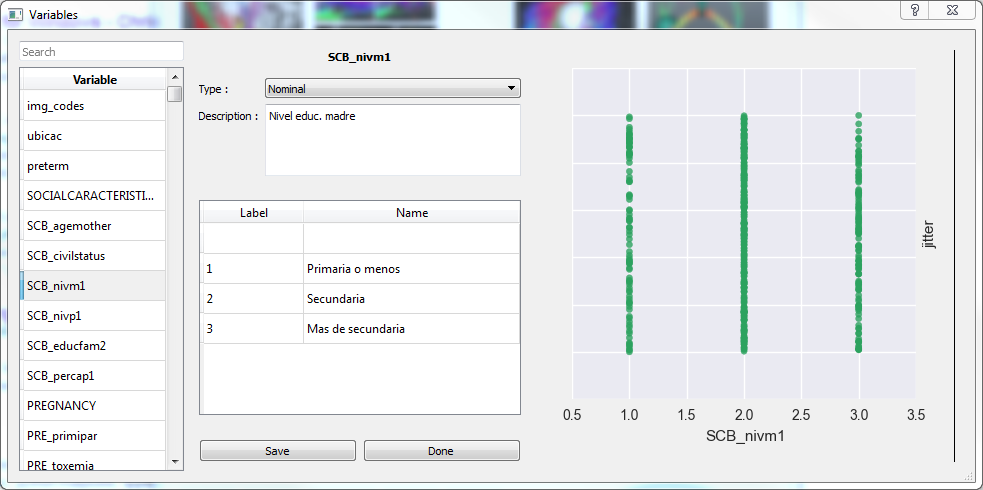
\includegraphics[width=0.9\textwidth]{braviz_qt/var_select.png} 
\caption{\label{fig_var_select}The standard dialog for selecting variables, notice the middle panel contains information about the variable while the right plot provides an overview.}
\end{figure}

The database of variables is a central component of this version, and as such we added features to perform typical statistical analyses on them without having to leave the platform. Figure \ref{fig_anova_2} shows an interface for performing anova  analysis using the data on the database. The user just selects an outcome, regressors, interactions and a sample. Samples can be created by filtering the population or other samples. An important advantage of doing the analysis here is that points in plots are also coordinated with other applications. This means that it is possible to right click on a point in a plot and make all currently open applications focus on that subjects, this includes the \emph{subject overview} application.

\begin{figure}
\centering
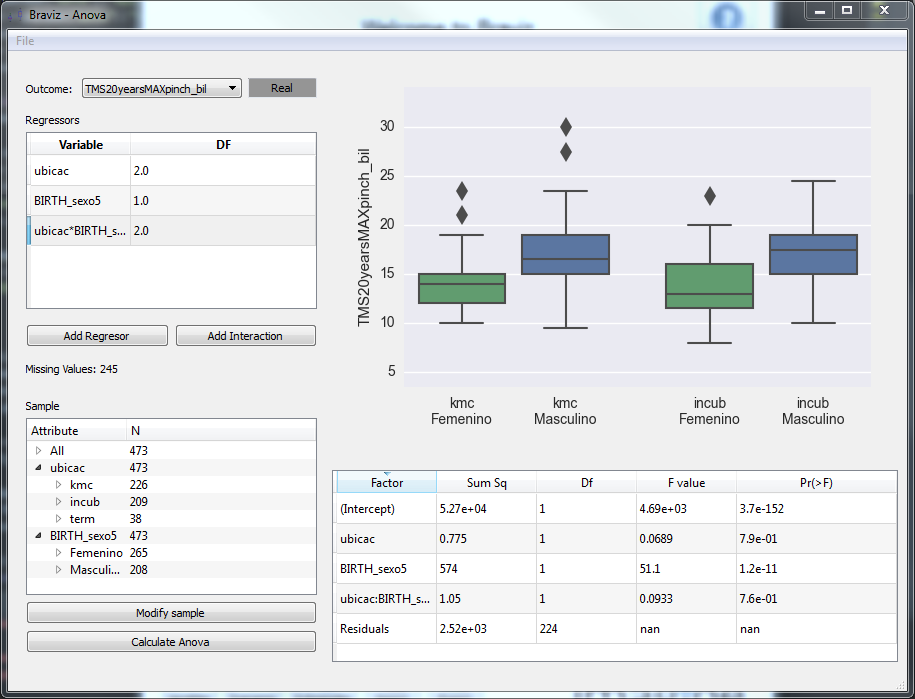
\includegraphics[width=0.9\textwidth]{braviz_qt/anova.png} 
\caption{\label{fig_anova_2}Anova analyzes on the variables in the database can be performed and visualized on this application. Data-points in the plots are coordinated to all other open applications.}
\end{figure}

Figure \ref{fig_lm_2} shows a similar application tuned for linear regressions. In this nominal variables are encoded using dummy variables, and the effects of each variable can be analyzed in the presence of the other variables. 

\begin{figure}
\centering
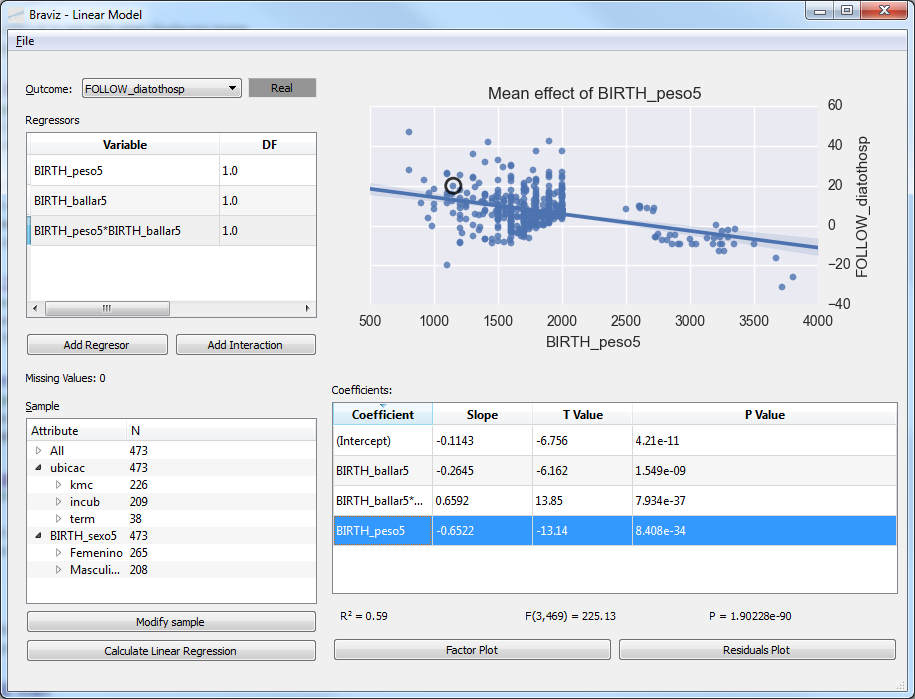
\includegraphics[width=0.9\textwidth]{braviz_qt/linear_model.png} 
\caption{\label{fig_lm_2}An application for fitting linear models on the variables on the database, the effect of one variable after correcting for the others can be visualized. Notice the highlighted subject in the plot.}
\end{figure}

Finding correlations between variables is a common task for researchers, and thus we developed the application shown in figure \ref{fig_correlations}. It features a correlations matrix in the middle, on the left side is a list of all variables in the project which can be added or removed from analysis with a click. Finally, when the user clicks on a square of the matrix a scatter plot of the two variables is shown at the right. This scatter plot also allows users to select a point and see the corresponding subject on other views, and it reacts to messages sent for this purpose from other applications. Another feature is that individual points can be added or removed from the sample just by clicking on them, in this way anormal points that have a large influence on the regression can be temporarily removed from the analysis. The reduced sample that is created trough this process can be shared to other applications to perform other analysis.

\begin{figure}
\centering
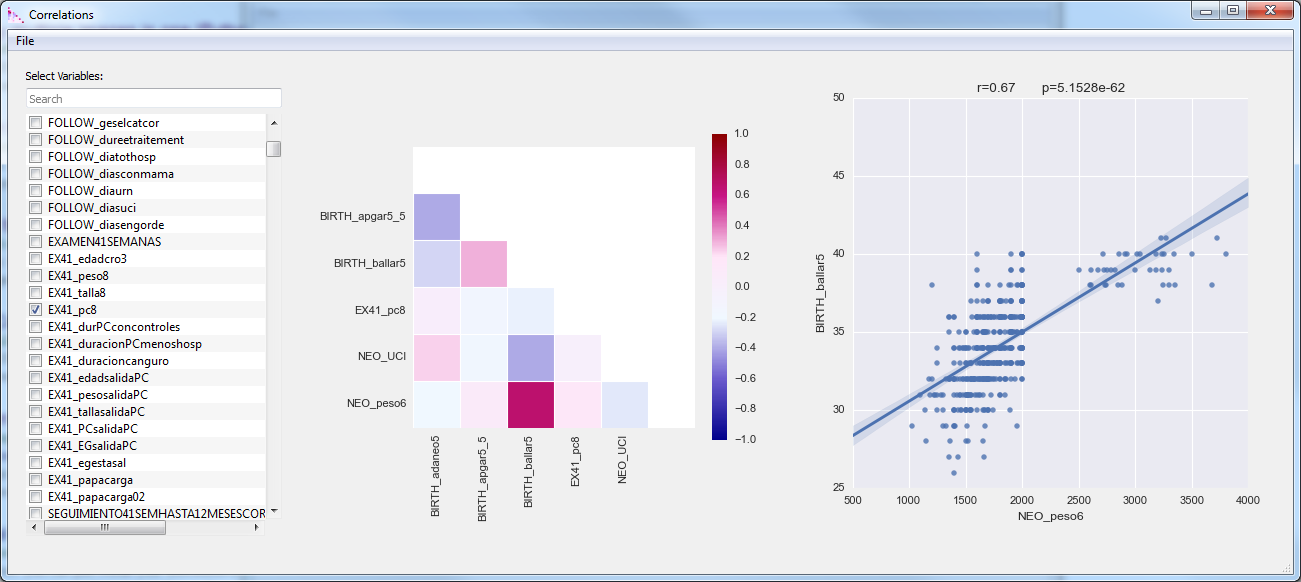
\includegraphics[width=0.9\textwidth]{braviz_qt/correlations.png} 
\caption{\label{fig_correlations}With this application it is straightforward to analyze correlations between variables.}
\end{figure}

The fMRI viewer from the previous iteration was upgrade to the one shown on figure \ref{fig_fmri_2}. This new version now loads complex experiment designs and contrasts directly from SPM files, which gives instantaneously an intuition of experiment structure, and makes mistakes evident. The new application also lets the user select multiple timelines at the same time, group them together, and make comparisons between groups. 

\begin{figure}
\centering
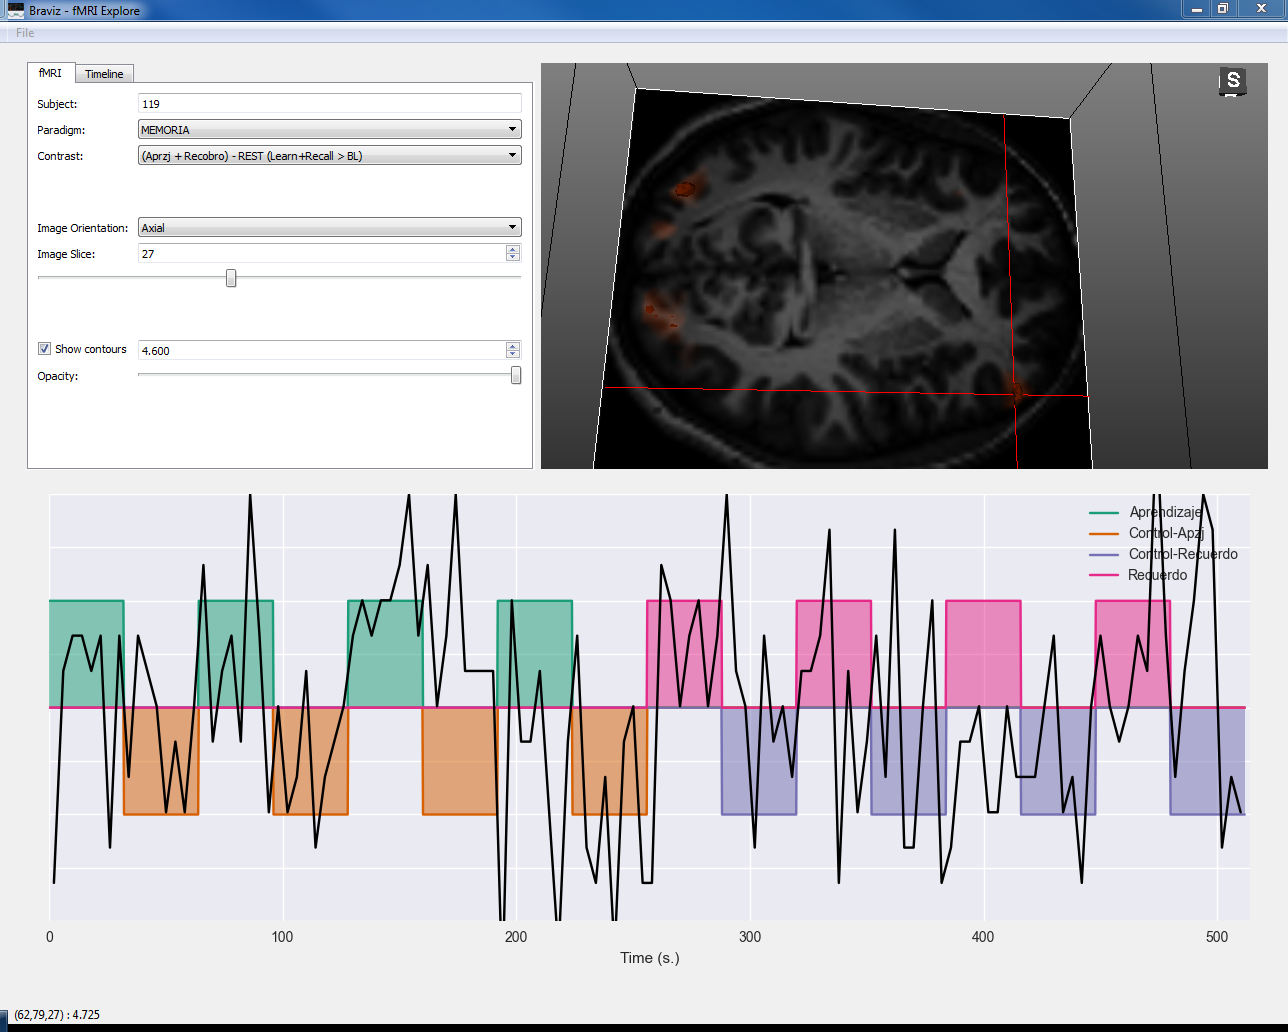
\includegraphics[width=0.9\textwidth]{braviz_qt/fmri.png} 
\caption{\label{fig_fmri_2}New version of the fmri explorer, now more complex experiments can be analyzed and timelines from different locations and subjects can be saved and compared.}
\end{figure}

While most of the applications of this iteration use QT for the graphical interface, we were also interested in web based technologies. Figure \ref{fig_parallel_2} shows a parallel coordinates view of the variables in the database created with the D3 \autocite{bostock_d$^3$_2011} javascript library and running on a web browser. Each line on the visualization represents a subject, while each axis represents a variable. Even though this application is running on a web browser, it is still possible to synchronize it with the rest of the system. This means the user can right click on one of the lines and make all the other apps focus on that subject, and in the same way, a line will be highlighted when the user asks for so in any other application. The mechanisms for making this possible will be explained on section \ref{sec_tech}.

\begin{figure}
\centering
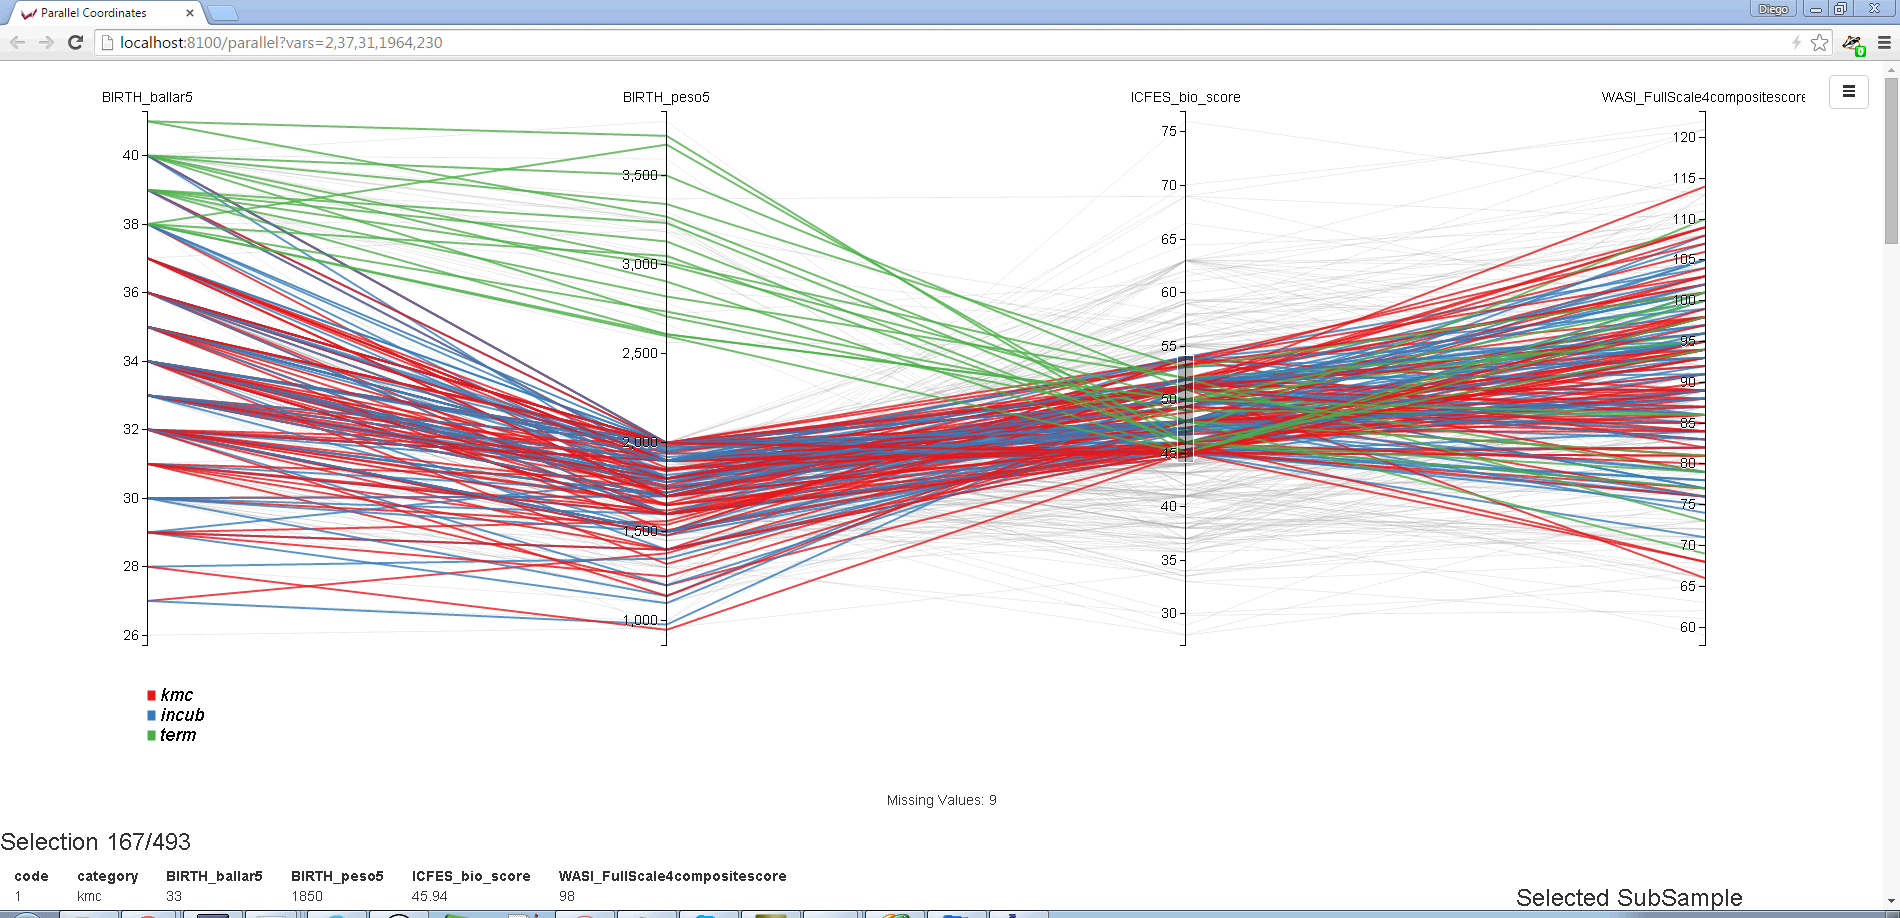
\includegraphics[width=0.9\textwidth]{braviz_qt/parallel.png} 
\caption{\label{fig_parallel_2}A parallel coordinates view of the variables in the database. Notice this visualization runs on a web browser.}
\end{figure}

Finally the menu, which acts as the entry point to the system, was also upgraded. Now in addition to the application launchers it includes utilities to import data into the database and export it, review and modify subsamples, look at the current variables and their meta-data, and review the saved states (scenarios) for all applications. From this last menu, it is possible to open any scenario, the correct application will then launch and load the saved state. Notice that the menu includes a first row with applications dedicated to manual or semi-manual measuring tasks. The objective of these applications is defining new geometrical structures or scalar measures that can be used in the rest of the system. It is possible to make linear measures on top of images, place spherical regions of interest based on images or surfaces while looking at the set of fibers that would result from that selection, and define custom fiber bundles by combining spheres and segmented structures trough logical operations. Examples of this will be given on chapter \ref{chap_kmc}.

\begin{figure}
\centering
\includegraphics[width=0.4\textwidth]{braviz_qt/braviz_menu.png} 
\caption{\label{fig_menu_2}The menu for the new version of Braviz, notice the utilities on the bottom row.}
\end{figure}

% Sample applications
% Maybe recycle from paper , or from old draft on bitbucket


\section{Architecture}
\label{sec_arch}

%From model to implementation
%-----------------------------
%
%- architecture
%- common platform
%- coordinate system
%- skeleton of a application
%- database


Trough the user centered design process described in the previous section we arrived to the model described on chapter \ref{chap_model}. The proposal consists of a family of applications, each providing interfaces, visualizations and interaction mechanisms suited for specific tasks. However all applications share the same data and can communicate with other running applications. While they will be different from the user point of view, on the inside they share several operations, therefore it makes sense for them to share significant amounts of code. Another important requirement was that the whole system should adapt to different data storage mechanisms. 

The proposed architecture to implement these features is shown in figure \ref{fig_archi}. At the top of the diagram are the concrete applications. All of them make use of a library which provides all common braviz functionalities. Notice that each application can use a different subset of features from this library, as specified in figure \ref{fig_feature_solution}. In order to made the platform flexible, and adaptable to different data storage solutions, all data access operations are isolated trough the "`Project Reader"' layer. The current implementation uses files stored in disk, but we had used this layer to adapt to two different disk layouts. In the future this layer could be used to read spatial data from a database or web service. 

\begin{figure}
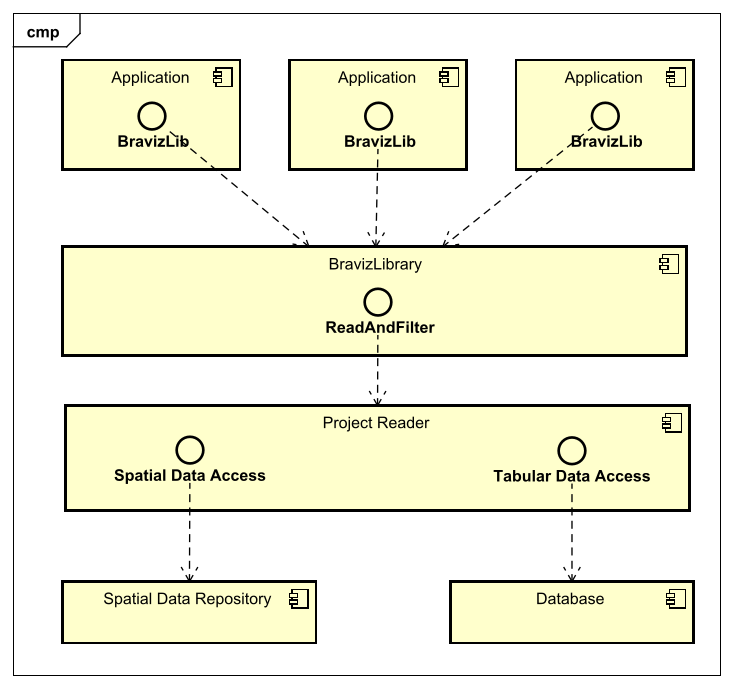
\includegraphics[width=\textwidth]{braviz/appArchitecture}%
\caption{\label{fig_archi} The architecture of Braviz Applications. The bottom of the diagram shows the underlying data storage, which is expected to be different for every project. The "`Project Reader"' layer serves as an isolation layer, when data storage mechanisms change only this layer needs to be adapted.}
\end{figure}

The library itself is divided into three modules

\begin{itemize}
	\item Read and Filter: Provides functions to access data and manipulate spatial data. This module loads the appropriate project reader based on a configuration file. However project readers themselves can use the other facilities in the module in order to transform the data into the expected format.
	\item Interaction: Provides re-usable widgets and interaction mechanisms, including communications with other applications in the family.
	\item Visualization: Provides several visualization elements, both for spatial data and tabular data.
\end{itemize}



\subsection{Read and Filter}

The \emph{readAndFilter} modules is in charge of providing the right data for all the other components. This mainly corresponds to the \emph{Data Sources} feature in\ref{fig_feature_solution}, and some basic \emph{Geometric Processing} operations, mainly related to data filtering and coordinate space transformation. 

Spatial data is exposed to the top layers via a declarative API; where the type of data, subject, coordinate system, and other parameters appropriate for the data type are passed to a function. Inside the function loads and applies all the required transformations. Each project reader must implement this API and must do the concrete operations required in the specific data-set to return the requested objects. Some examples of a call to this function can be seen in listing \ref{listing_read_and_filter_api}.

\begin{listing}
\inputminted{python}{code/read_and_filter_1.py}
\caption{Example of the Braviz spatial data reader API}
\label{listing_read_and_filter_api}
\end{listing}

The complete documentation can be found on the Braviz website. Notice that changing the coordinate system or the current subject is trivial if variables are used as arguments in all queries. Readers can also implement caching mechanisms in order to improve performance of future queries.  

Notice that it is possible to request specific sets of fibers by setting way-points in the query. This mechanism only supports getting bundles of fibers that cross several way-points or which cross any of them. More complex bundles can be requested by implementing specific functions inside the project reader, or by reading its description from the database. 

The types of data available for each project is not always the same. For this reason this method must also be able to inform applications which kinds of data are available. For this purpose most data types include an index parameter as can be seen on listing \ref{listing_read_and_filter_indices}.

\begin{listing}
\inputminted{python}{code/read_and_filter_indices.py}
\caption{Getting lists of available data}
\label{listing_read_and_filter_indices}
\end{listing}

Applications and functions from other modules may assume that this function exists and behaves as expected, and in this way applications that work across different projects can be built. This API can also be used in an interactive console in order fetch data on the fly.

Project readers themselves are likely to share several operations. For this reason the module provides reusable functions wrapping input and output, format changes, transformations between coordinate systems and computation of scalars.

The spatial data repository should not be writable by the Braviz system. In this way users won't fear altering their raw data while using Braviz, and the platform will be easier to use together with other systems. However there should be another location where the results from expensive operations can be stored in a persistent cache. 

Complementing this source of spatial data is a database which contains several objects which can be manipulated by end users. This include

\begin{itemize}
\item Variables values and metadata
\item Saved application state
\item Subsamples
\item Subject Annotations
\item User defined fiber bundles
\item User defined geometrical objects (ROIs, Lines)
\end{itemize}

The concrete way in which these objects are stored depends on the project, but all reading and writing into the database should also be limited to this modules. More details about the currently implemented schema will be given in section \ref{sec_tech}


\subsection{visualization}

The visualization module provides reusable interactive visualizations. These are divided in two families: spatial data viewers based on VTK and statistical data viewer based on Matplotlib or D3. 

Spatial data viewers are made from several \emph{managers} specialized for dealing with each of the different data types. All managers draw to the same renderer, but each of them keeps the objects associated to specific kinds of data. In order for the full viewer to behave correctly it is important to keep all managers in the same coordinate system and the same subject. The currently available managers are 

\begin{itemize}
	\item ImageManager: Displays an image in a plane. The user can click on the image to get the values and coordinates of the current voxel. The manager keeps track of the current image modality, orientation and slice.
	\item FmriContours: Displays contoures for fMRI statistical maps. The manager keeps track of the paradigm and contrast, and the level of the template. A custom lookup-table can be used to color the contours.
	\item Model Manager: Displays segmented structures. Keeps tracks of the available models and the currently selected models. Can also return scalar values associated to the current models, and allows specifying models by laterality ("`dominand or non-dominant"') or side ("`left"' or "`right"').
	\item SurfaceManager: Displays freeSurfer surface reconstructions and its associated scalars. As the model manager it can handle subject laterality. Users can click on top of the cortical surfaces and get the value of the associated scalar. 
	\item TractographyManager: Displays tractography bundles colored according to direction, fa, md or using one different color for each bundle. Bundles can be defined using a list of models joined by \emph{and} or \emph{or}, or loaded from the database. 
	\item TraculaManager: Displays tracula bundles as surfaces.	
	\item Others: spheres, lines, planes or other objects should be in separate managers.
\end{itemize}

Concrete viewers are created by adding the required managers and writing the code that coordinates them. Also not all of the available configurations of each manager need to be exposes. This provides flexibility to create a viewer fit for each application.


For statistical visualization a qt widget the library provides a qt-widget that can display scatter plots, box plots, bar plots, and others. All of these implement tooltips and context menus for each data point and the ability to highlight a subject of group of subjects in the plot. Statistical visualizations can also be created using javascript libraries, specially D3. This is achieved by serving pages and data trough the Braviz web server. More details will be given in section \ref{sec_tech}.

\subsection{interaction}

The interaction module provides communication between applications and access to data processing functions. Communications are achieved by installing a communications client on each applications, which connects to a server usually found on the main menu application. Applications send messages trough the client, which are then relied to all running applications. When a message is received the client lets the application handle it. Currently there are a few types of messages available, but the protocol allows easy extensions

\begin{itemize}
\item Subject: Indicates applications that they should switch focus towards a particular subject
\item Sample: Indicates applications that they should work with different sub-sample
\item Log: Communicates the system of important user actions that should be stored into the analysis log
\end{itemize}


Statistical data processing is achieved by calling \emph{R} functions trough the rpy2 interface. All associated \emph{R} code should is contained in this module. Currently the available operations are restricted to fitting anova and linear models and calculating the importance of each variable towards predicting another by using a random forest model. New functions will be added to this module as they are required by applications. 

Spatial data can be processed using VTK, python scientific libraries or both. Currently the module provides functions to calculate values of an image inside a surface and calculating geometric descriptors of surfaces as volume or lengths of main axes.

This module also provides several Qt models, dialogs and widgets that can be reused on applications. This includes dialogs for saving and loading samples and scenarios and for selecting variables. Models are available to represent samples and structures. Finally there are convenience widgets for common applications as selecting samples or selecting images and fMRI paradigms and contrasts.

\subsection{applications}

The applications that are currently part of the system are listed below, together with its main components. This will show how the variability of the system can be materialized into a wide arrange of applications. 

\begin{itemize}

\item \emph{Roi Builder}: Lets the user define spherical ROIs using images or cortices as context. It includes a 3D viewer which can display images in 3-orthogonal planes, brain cortices, a sphere and the fiber bundles that go trough the sphere. It can provide the mean value of an image inside the current ROI. ROI locations for different subjects can be approximated by making use of registered coordinate systems.

\item \emph{Linear Measure}: Lets the user make linear measures on top of an image. It provide a viewer with three orthogonal planes and a line defined on top of a certain plane.

\item \emph{Logic Bundles}: Lets the user define fiber bundles by combining ROIs and segmented structures with logical operations (\emph{and}, \emph{or} and \emph{not}). It provides a 3D viewer where the bundle can be previewed together with tree orthogonal planes and brain cortices. Scalars associated with the bundle can be calculated.

\item \emph{Subject Overview} (Figure \ref{fig_subj_overview_2}): Provides a fully configurable 3D viewer with images, segmented structures, fMRI contours, tractography, Tracula bundles and cortical surfaces. It can calculate scalars from bundles or segmented structures. Also provides annotations and values for the current subject on selected variables. Communicates to other applications when the current subject changes and responds to subject messages by switching to that subject.

\item \emph{Sample Overview} (Figure \ref{fig_sample_overview_2}): Provides multiple 3D viewers which are associated to different subjects together with a bar plot. The configuration of each viewer is copied from one created in \emph{Subject Overview}. Viewers are arranged in a grid where columns are levels of a nominal variable and sorted from left to right based on a numerical variable. Bars are connected to the corresponding viewer. By right clicking on a subject either on a subject or bar, it is possible to communicate to other applications that they should focus on it. The applications also reacts to subject messages by highlighting the given subject.

\item \emph{Explore fMRI} (Figure \ref{fig_fmri_2}): Includes a 3D viewer that shows an fMRI image and contours. At the bottom is a time-line which shows the current contrast and the bold signal associated with the current coordinates. It is possible to get this signals from multiple locations or multiple subjects. This signals can later be grouped together in order to compare patterns between groups. The application communicates subject changes and switches to a subjects when asked to by a message.

\item \emph{Check Registration}: Provides a viewer with a single plane where two different images can be viewed using a checkerboard pattern. 

\item \emph{Anova} (Figure \ref{fig_anova_2}): Lets the user fit Anova models based on variables in the database. Provides an statistical viewer that can show box plots, scatter plots or Anova diagnostics. By right clicking on a point in the plot the user can communicate to other applications that they should switch focus to the corresponding subject. When a subject message is received, the corresponding message will be highlighted in the plot.

\item \emph{Linear Model} (Figure \ref{fig_lm_2}): Lets the user fit linear models where nominal variables with more than two levels are encoded using dummy variables. It has a statistical plot that can show scatter plots, diagnostics or regression plots. The plot can be used for communications in the same way as the one in \emph{Anova}.

\item \emph{Correlations} (Figure \ref{fig_correlations}): Displays a correlation matrix with selected variables and scatter plots with correlation values. In the scatter plots subjects can be removed or added back to the analysis. The modified sample can be shared with other applications. The scatter plot also includes the communication properties of the \emph{Anova} plot.

\item \emph{Parallel Coordinates} (Figure \ref{fig_parallel_2}): This application provides a D3-based parallel coordinates display with variables from the database. Filters can be applied on each axis and the resulting sample can be shared with other running applications. It is also possible to right click on a line in order communicate other applications they should focus on that subject, likewise the application will receive subject messages and highlight the indicated subject.

\end{itemize}

All but \emph{Parallel Coordinates} are stand alone Qt applications. However in the future we expect to have more web based applications. Also notice all of them can save and restore their state from the database. Applications with a concept of sample can save and load samples into the database. They also provide access to the sample creation dialog where samples can be modified. Sharing samples to all applications requires explicit actions in the part of the user, as otherwise this could be disturbing. On each application users can choose if they always accept received samples, always reject them, or ask every time. 

Chapter \ref{chap_kmc} will show examples of how this applications are used in a real project. This will clarify the role each of them play and how instant communication can enhance analysis.

%¿Maybe a table indicating which features are used in each application?

%Show variability

\section{Technical Details}

\label{sec_tech} 

Technical details
------------------

- libraries
- data input/output
- messaging protocol
- transformations
- coordinate systems
% Dibujo esquema base de datos


